\chapter{THE HEAVY ELEMENTS}
% !TEX root = hazy3.tex

\section{Overview}

The code considers all 465 atoms and ions of the lightest 30 elements.
The treatment of the ionization equilibrium of ions with more than two
electrons is conventional (see AGN3).  This treatment is more approximate
than that of the H and He iso-sequences because the majority of ions are
treated considering only the ground term and continuum for each ionization
stage.  In all cases, collisional ionization from ground and a net three-body
recombination coefficient are included.
Photoionization rates are modified
for induced recombination as described by equation~\ref{eqn:InducedRecombinationRateCoefficient}.
All published charge transfer rate coefficients are also included
\citep{Kingdon1996}.  Inner shell photoionization is treated using
Auger yields given by \citet{Kaastra1993}.  Photoionization cross
sections are from \citet{VernerFerlandKorista1996}.

This treatment is approximate at high densities for two reasons.  First,
net radiative recombination coefficients, which have been summed over all
levels are used.  These sums are correct only in the low-density limit.
At high densities levels can undergo collisional ionization before radiative
decays to the ground state occur.  This brings high levels into LTE, which
actually increases the recombination rate.  A second problem is that
substantial populations can build up in highly excited states when the
density and temperature are high.  When this occurs, the partition function
of the atom or ion is no longer equal to the statistical weight of the ground
state.  As a result the ionization equilibrium of the heavy elements is
approximate for very high densities $(n \gg 10^{10} \mathrm{cm}^{-3})$, with uncertainties
increasing for higher densities.  The statistical and thermal equilibrium
of high-density gas is an area of on-going research.

Many exotic line transfer effects can influence certain lines due to
coincidental line overlap.  A good general reference to a number of these
processes is the paper by \citet{Swings1940}.  All of these processes
are included in the line formation processes for those lines that are
predicted by the code.  \citet{Morton1988} and
\citet{VernerVernerFerland1996} provide a line list for UV resonance lines, and \citet{Bowen1960}'s
paper on forbidden lines remains a classic.

The effects of resonant structures often dominate collision strengths
for infrared transitions.
\citet{Oliva1996} and \citet{VanHoof2000a} stress the uncertainties these may introduce.

\section{Solar system abundances}

Figure \ref{fig:SolarSystemAbundances} plots the solar system abundances of the elements, as tabulated
by \citet{Allende2001}, \citet{Allende2002},
\citet{Holweger2001} and \citet{Grevesse1998}.
The independent variable is the abundance by number relative to a scale where
the abundance of silicon is 10$^6$.  The dependent vaariable lists the atomic number and
the chemical symbol for the element.

\begin{figure}
\centering
\label{fig:SolarSystemAbundances}
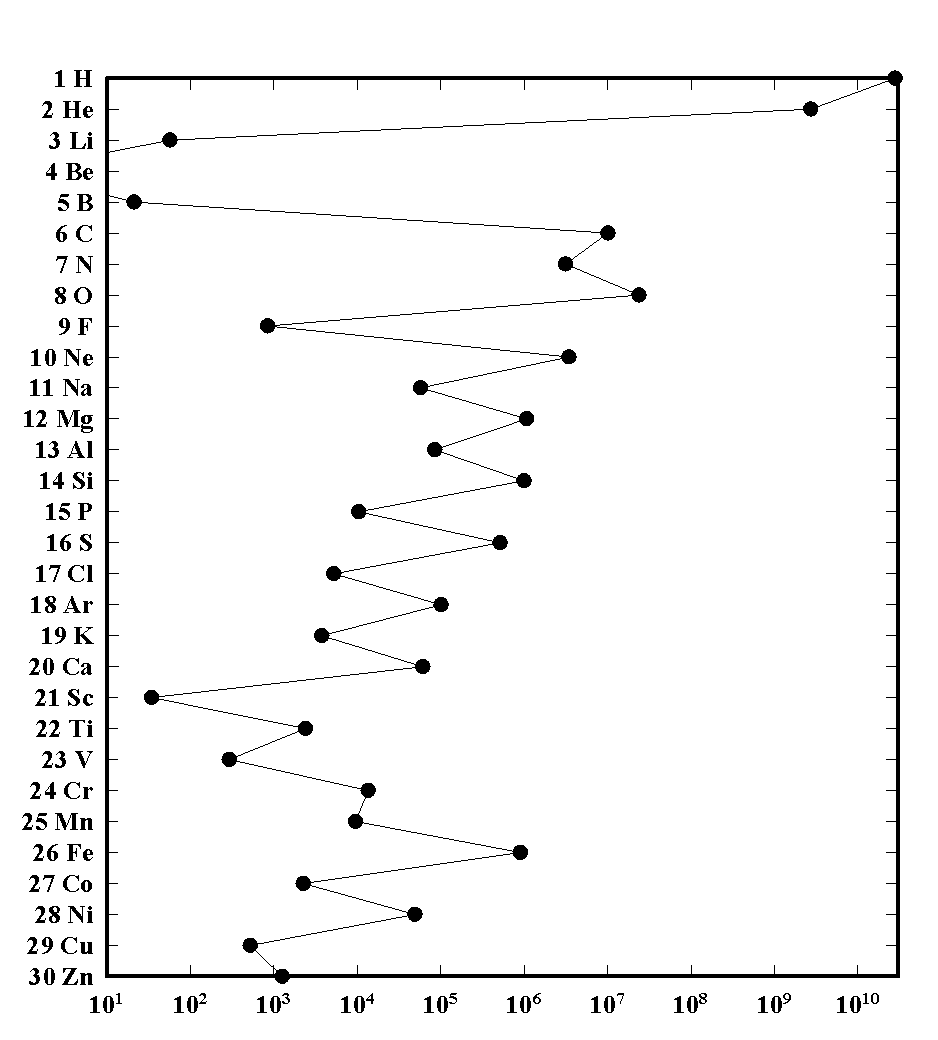
\includegraphics[scale=0.7]{SolarSystemAbundances}
\caption[Solar system abundances]{Solar system abundances are shown.}
\end{figure}

\section{Periodic table}

A periodic table of the first 36 elements follows.

\begin{tabular}{lllllllllllllllllll}
\hline
1&&&&&&&&&&&&&&&&&2\\
H&&&&&&&&&&&&&&&&&He\\
3&4&&&&&&&&&&&5&6&7&8&9&10\\
Li&Be&&&&&&&&&&&B&C&N&O&F&Ne\\
11&12&&&&&&&&&&&13&14&15&16&17&18\\
Na&Mg&&&&&&&&&&&Al&Si&P&S&Cl&Ar\\
19&20&21&22&23&24&25&26&27&28&29&30&31&32&33&34&35&36\\
K&Ca&Sc&Ti&V2&Cr&Mn&Fe&Co&Ni&Cu&Zn&Ga&Ge&As&Se&Br&Kr\\
\hline
\end{tabular}

\section{Ionization balance}

\subsection{Photoionization cross sections}

Photoionization cross sections for all elements are evaluated using Dima
Verner's fits to Opacity Project data where possible, and the best
theoretical or experimental data for other cases.
The fitting procedure
is described in \citet{Verner1993}, \citet{Verner1995},
and \citet{VernerFerlandKorista1996}.

\subsection{Auger multi-electron ejection}

Many electrons may be ejected following removal of an inner electron.
This is fully treated using electron yields taken from
\citet{Kaastra1993}.
This process couples non-adjacent stages of ionization.

Figure \ref{fig:IronPhoto} shows photoionization cross sections for each shell of singly
ionized iron, along with plots of the electron yield, assuming data given
by \citet{Kaastra1993}.  A single photoionization of the 1s shell can
remove as many as 8 electrons.

\begin{figure}
\centering
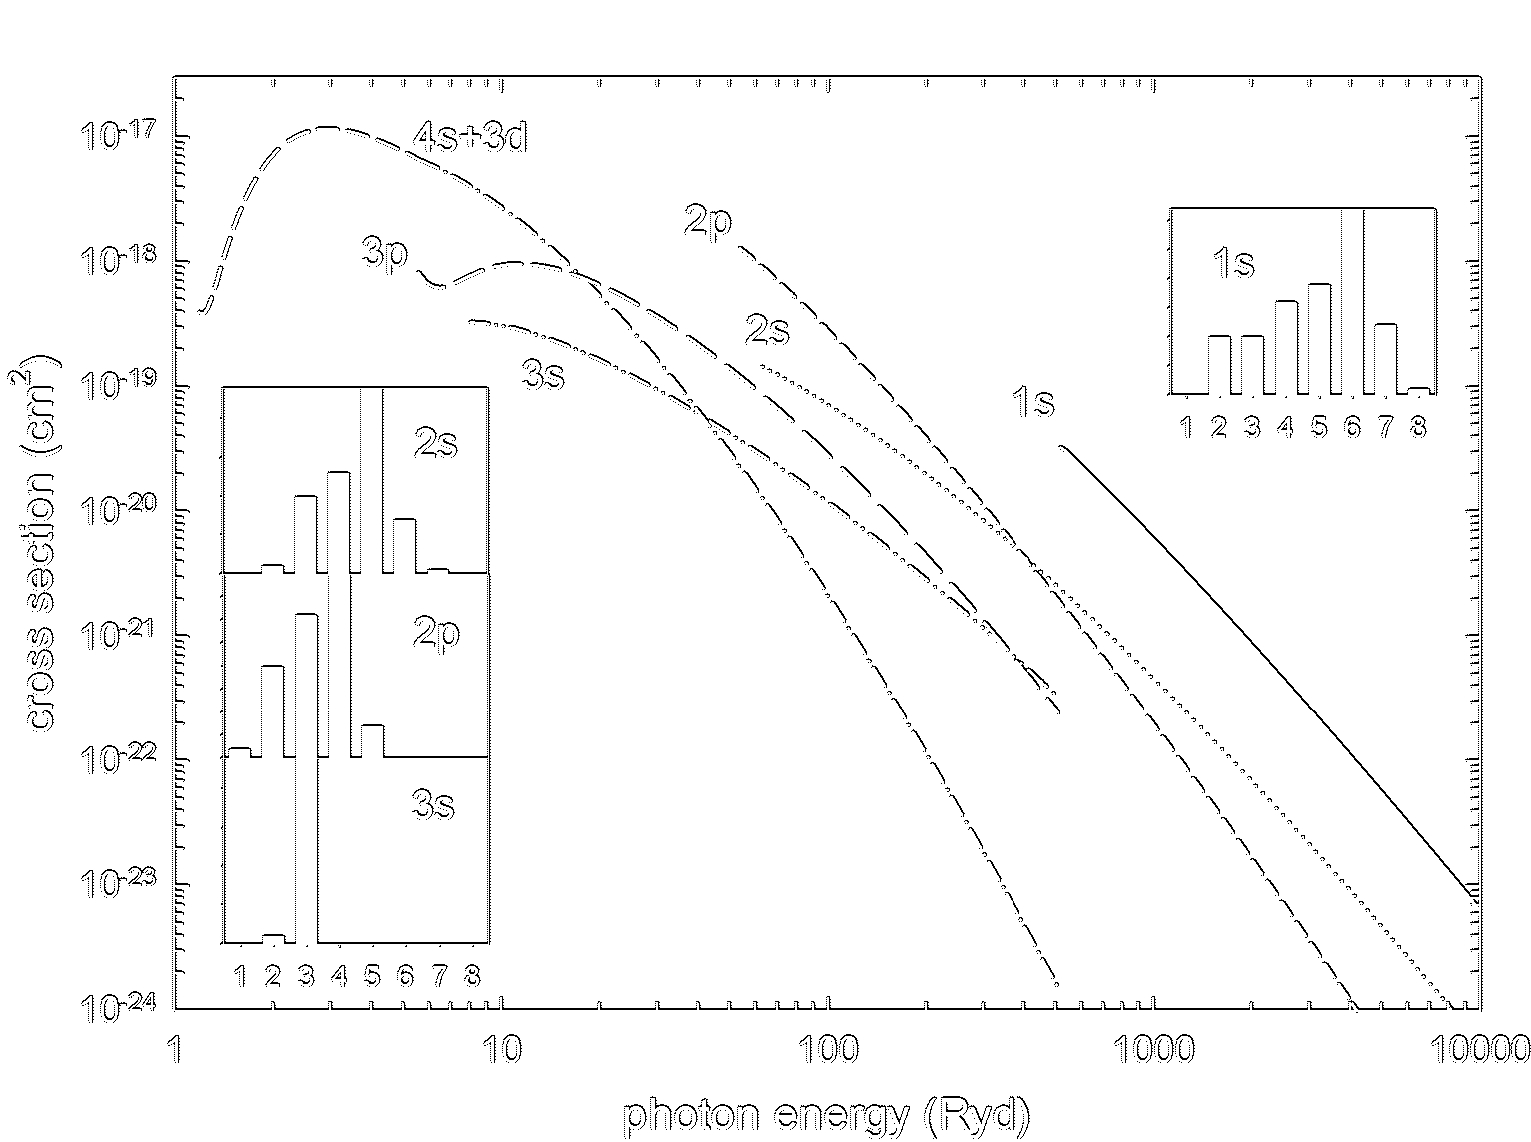
\includegraphics[scale=0.6]{IronPhoto}
\caption[Photoionization cross sections and yields for Fe$^+$]
{Photoionization cross sections and electron yields for singly
ionized iron.  Each subshell is shown along with the corresponding electron
yield.}
\label{fig:IronPhoto}
\end{figure}

\subsection{Compton scattering ionization of bound electrons}

Ionization of outer valence electrons by Compton scattering is treated
for all species by assuming that the cross section is the relativistic
Compton cross section, multiplied by the number of valence electrons.

\subsection{Collisional ionization rate coefficients}

Fits to collisional ionization rate coefficients are evaluated in Dima
Verner's routine \cdRoutine{cfit}.
These rates come mainly from \citet{Arnaud1992}
and \citet{Arnaud1985}, and by interpolation where rates
are not given.

\subsection{Charge transfer}

Rates for charge transfer between hydrogen and the heavy elements are
evaluated using Jim Kingdon's routines.   For species more than 4 times
ionized, a statistical estimate made by Alex Dalgarno (\citealp{Ferland1997})
is used.  The rate coefficient for transfer between atomic hydrogen and
a highly ionized species is given by
$1.92\times 10^{-9} \; \zeta \; \pcc \ps$,
where $\zeta$ is the
charge of the ion.  Other atoms are treated analogously.

All of these include the thermal effects of charge transfer, as described
by \citet{Kingdon1998b}.

\section{Ionization potentials}

Table \ref{tab:IonizationPotentials} lists ionization potentials for photoionization of the outer
shell of the first thirty elements.  These are given in Rydbergs for infinite
mass nuclei.

\begin{table}
\scriptsize
\caption{Ionization Potentials of the Elements (Rydbergs)}
\label{tab:IonizationPotentials}
\begin{tabular}{lllllllllll}
\hline
&1 H& 2 He& 3 Li& 4 Be& 5 B& 6 C& 7 N& 8 O& 9 F& 10 Ne\\
\hline
1& 9.996(-1)& 1.807& 3.963(-1)& 6.852(-1)& 6.099(-1)& 8.276(-1)& 1.068&
1.001& 1.280& 1.585\\
2&& 4.000& 5.559&
1.338& 1.849& 1.792& 2.176& 2.581& 2.570& 3.010\\
3&&&  9.003& 1.131(+1)& 2.788& 3.520&
3.487& 4.038& 4.609& 4.664\\
4&&&&  1.600(+1)& 1.907(+1)& 4.740& 5.694& 5.689& 6.405& 7.138\\
5&&&&&  2.500(+1)& 2.882(+1)& 7.195& 8.371& 8.393& 9.275\\
6&&&&&&
3.601(+1)& 4.058(+1)& 1.015(+1)& 1.155(+1)& 1.161(+1)\\
7&&&&&&& 4.903(+1)& 5.434(+1)& 1.361(+1)& 1.524(+1)\\
8&&&&&&&& 6.405(+1)& 7.011(+1)& 1.757(+1)\\
9&&&&&&&&& 8.107(+1)& 8.790(+1)\\
10&&&&&&&&&& 1.001(+2)\\
\hline
\end{tabular}
\end{table}

\begin{table}
\scriptsize
\caption{Ionization Potentials of the Elements (Rydbergs)}
\begin{tabular}{lllllllllll}
\hline
&11 Na& 12 Mg& 13 Al& 14 Si& 15 P&16 S& 17 Cl& 18 Ar& 19 K& 20 Ca\\
\hline
1&
3.777(-1)&5.620(-1)&4.400(-1)&5.991(-1)&7.710(-1)&7.614(-1)&9.533(-1)&1.158&
3.191(-1)&4.493(-1)\\
2& 3.476& 1.105& 1.384& 1.202& 1.450& 1.715& 1.750& 2.031& 2.325&
8.724(-1)\\
3& 5.264& 5.890& 2.091& 2.461& 2.220& 2.560& 2.911& 2.994& 3.367& 3.742\\
4& 7.270&
8.033& 8.820& 3.318& 3.781& 3.477& 3.930& 4.396& 4.477& 4.944\\
5& 1.017(+1)& 1.039(+1)& 1.130(+1)& 1.226(+1)& 4.780& 5.342& 4.985& 5.514&
6.075& 6.211\\
6& 1.266(+1)& 1.371(+1)& 1.400(+1)& 1.507(+1)& 1.620(+1)& 6.471& 7.131&
6.689& 7.309& 7.996\\
7& 1.532(+1)& 1.653(+1)& 1.774(+1)& 1.812(+1)& 1.934(+1)& 2.065(+1)& 8.393&
9.136& 8.643&
9.349\\
8& 1.942(+1)& 1.955(+1)& 2.092(+1)& 2.228(+1)& 2.274(+1)& 2.412(+1)&
2.560(+1)& 1.055(+1)& 1.137(+1)& 1.082(+1)\\
9& 2.204(+1)& 2.412(+1)& 2.426(+1)& 2.580(+1)& 2.732(+1)& 2.786(+1)&
2.941(+1)& 3.105(+1)& 1.292(+1)& 1.384(+1)\\
10& 1.077(+2)& 2.701(+1)& 2.935(+1)& 2.950(+1)& 3.120(+1)& 3.286(+1)&
3.349(+1)& 3.518(+1)& 3.703(+1)& 1.553(+1)\\
11& 1.212(+2)& 1.295(+2)& 3.249(+1)& 3.499(+1)& 3.525(+1)& 3.710(+1)&
3.890(+1)& 3.961(+1)& 4.150(+1)& 4.350(+1)\\
12&& 1.443(+2)& 1.533(+2)& 3.848(+1)& 4.119(+1)& 4.150(+1)& 4.351(+1)&
4.544(+1)& 4.627(+1)& 4.830(+1)\\
13&&&  1.693(+2)& 1.792(+2)& 4.497(+1)& 4.790(+1)& 4.827(+1)& 5.043(+1)&
5.253(+1)& 5.341(+1)\\
14&&&& 1.965(+2)& 2.070(+2)& 5.198(+1)& 5.511(+1)& 5.555(+1)& 5.782(+1)&
6.010(+1)\\
15&&&&& 2.256(+2)& 2.370(+2)& 5.949(+1)& 6.283(+1)& 6.329(+1)& 6.575(+1)\\
16&&&&&& 2.568(+2)& 2.689(+2)& 6.747(+1)& 7.115(+1)& 7.162(+1)\\
17&&&&&&& 2.900(+2)& 3.029(+2)& 7.607(+1)& 7.989(+1)\\
18&&&&&&&& 3.253(+2)& 3.389(+2)& 8.504(+1)\\
19&&&&&&&&& 3.626(+2)& 3.770(+2)\\
20&&&&&&&&&& 4.020(+2)\\
\hline
\end{tabular}
\end{table}

%   Table 1c
\begin{table}
\scriptsize
\caption{Ionization Potentials of the Elements (Rydbergs)}
\begin{tabular}{lllllllllll}
\hline
& 21 Sc& 22 Ti& 23 V& 24 Cr& 25 Mn& 26 Fe& 27 Co& 28 Ni& 29 Cu& 30Zn\\
\hline
1& 5.396(-1)& 5.012(-1)& 4.954(-1)& 4.974(-1)& 5.464(-1)& 5.808(-1)&
5.780(-1)& 5.613(-1)& 5.678(-1)& 6.904(-1)\\
2& 9.408(-1)& 9.981(-1)& 1.077& 1.213& 1.149& 1.190& 1.255& 1.335& 1.491&
1.320\\
3& 1.820& 2.020& 2.154& 2.275& 2.475& 2.253& 2.462& 2.596& 2.708& 2.919\\
4& 5.401& 3.180& 3.433& 3.613& 3.763& 4.028& 3.768& 4.035& 4.217& 4.366\\
5& 6.752& 7.298& 4.798& 5.105& 5.321& 5.513& 5.843& 5.593& 5.872& 6.071\\
6& 8.136& 8.783& 9.415& 6.662& 7.037& 7.281& 7.497& 7.938& 7.570& 7.938\\
7& 1.014(+1)& 1.035(+1)& 1.107(+1)& 1.177(+1)& 8.768& 9.187& 9.481& 9.775&
1.022(+1)& 9.996\\
8& 1.162(+1)& 1.252(+1)& 1.275(+1)& 1.357(+1)& 1.430(+1)& 1.111(+1)&
1.160(+1)& 1.191(+1)& 1.227(+1)& 1.286(+1)\\
9& 1.323(+1)& 1.412(+1)& 1.513(+1)& 1.538(+1)& 1.630(+1)& 1.717(+1)&
1.368(+1)& 1.418(+1)& 1.463(+1)& 1.492(+1)\\
10& 1.654(+1)& 1.587(+1)& 1.694(+1)& 1.796(+1)& 1.825(+1)& 1.926(+1)&
2.024(+1)& 1.651(+1)& 1.705(+1)& 1.749(+1)\\
11& 1.836(+1)& 1.948(+1)& 1.879(+1)& 1.990(+1)& 2.102(+1)& 2.133(+1)&
2.244(+1)& 2.359(+1)& 1.956(+1)& 2.014(+1)\\
 12&5.052(+1)& 2.142(+1)&
2.264(+1)& 2.191(+1)& 2.311(+1)& 2.431(+1)& 2.469(+1)& 2.588(+1)& 2.711(+1)&
2.284(+1)\\
13& 5.562(+1)& 5.790(+1)& 2.472(+1)& 2.608(+1)& 2.525(+1)& 2.653(+1)&
2.786(+1)& 2.822(+1)& 2.947(+1)& 3.085(+1)\\
14& 6.106(+1)& 6.344(+1)&
6.585(+1)& 2.824(+1)& 2.962(+1)& 2.883(+1)& 3.021(+1)& 3.162(+1)& 3.197(+1)&
3.337(+1)\\
15& 6.817(+1)& 6.923(+1)& 7.172(+1)& 7.431(+1)& 3.199(+1)& 3.359(+1)&
3.263(+1)& 3.408(+1)& 3.557(+1)& 3.601(+1)\\
16& 7.416(+1)& 7.673(+1)& 7.791(+1)& 8.063(+1)& 8.327(+1)& 3.596(+1)&
3.763(+1)& 3.663(+1)& 3.822(+1)& 3.984(+1)\\
17& 8.041(+1)& 78.313(+1)& 8.584(+1)& 8.709(+1)& 8.996(+1)& 9.275(+1)&
4.017(+1)& 4.199(+1)& 4.094(+1)& 4.255(+1)\\
18& 8.915(+1)& 8.974(+1)& 9.261(+1)& 9.547(+1)& 9.680(+1)& 9.981(+1)&
1.027(+2)& 4.462(+1)& 4.652(+1)& 4.549(+1)\\
19& 9.466(+1)& 9.893(+1)& 9.959(+1)& 1.026(+2)& 1.056(+2)& 1.070(+2)&
1.106(+2)& 1.133(+2)& 4.929(+2)& 5.130(+1)\\
20& 4.171(+2)& 1.047(+2)& 1.093(+2)& 1.100(+2)& 1.131(+2)& 1.163(+2)&
1.178(+2)& 1.211(+2)& 1.242(+2)& 5.420(+1)\\
21& 4.435(+2)& 4.593(+2)& 1.154(+2)& 1.201(+2)& 1.208(+2)& 1.241(+2)&
1.275(+2)& 1.291(+2)& 1.318(+2)& 1.357(+2)\\
22&& 4.870(+2)& 5.036(+2)& 1.265(+2)& 1.314(+2)& 1.322(+2)& 1.357(+2)&
1.392(+2)& 1.400(+2)& 1.435(+2)\\
23&&& 5.326(+2)& 5.499(+2)& 1.382(+2)& 1.433(+2)& 1.441(+2)& 1.478(+2)&
1.503(+2)& 1.521(+2)\\
24&&&& 5.803(+2)& 5.983(+2)& 1.504(+2)& 1.557(+2)& 1.566(+2)& 1.597(+2)&
1.629(+2)\\
25&&&&& 6.300(+2)& 6.489(+2)& 1.631(+2)& 1.687(+2)& 1.689(+2)& 1.737(+2)\\
26&&&&&& 6.819(+2)& 7.015(+2)& 1.763(+2)& 1.807(+2)& 1.822(+2)\\
27&&&&&&& 7.357(+2)& 7.563(+2)& 1.900(+2)& 1.945(+2)\\
28&&&&&&&& 7.923(+2)& 8.129(+2)& 2.043(+2)\\
29&&&&&&&&& 8.504(+2)& 8.724(+2)\\
30&&&&&&&&&& 9.106(+2)\\
\hline
\end{tabular}
\end{table}

Figure \ref{fig:IonizationPotentials} shows the number of ions with valence shell ionization potentials
within logarithmically increasing energy widths, as a function of the log
of the ionization potentials in Rydbergs.  Two large peaks occur, one near
$\sim $25 Ryd ($\sim $350 eV) and a second near $\sim $160 Ryd ($\sim $2 keV).
The continuum binning used in the code is designed to resolve these as
separate features.

\begin{figure}
\centering
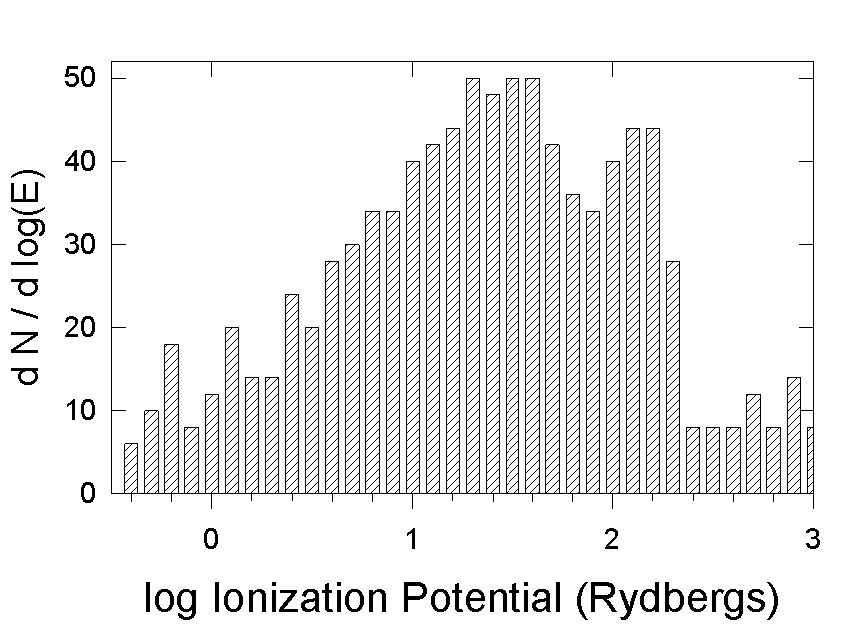
\includegraphics{IonizationPotentials}
\caption[Ionization potentials of the elements]{The number of elements with valence shell ionization potentials
within logarithmically increasing energy widths is shown as a function of
the log off the ionization potential.}
\label{fig:IonizationPotentials}
\end{figure}

\section{Isoelectronic sequences}

Figure \ref{fig:EnergyLevelsSecondRow} shows energy-level diagrams for second row iso-sequences.  For
sequences of elements heavier than K the ground configuration is correct
for ions twice or more times ionized.  For these heavier elements the atom
and first ion may have non-standard configurations for the outer shell.

\begin{figure}
\centering
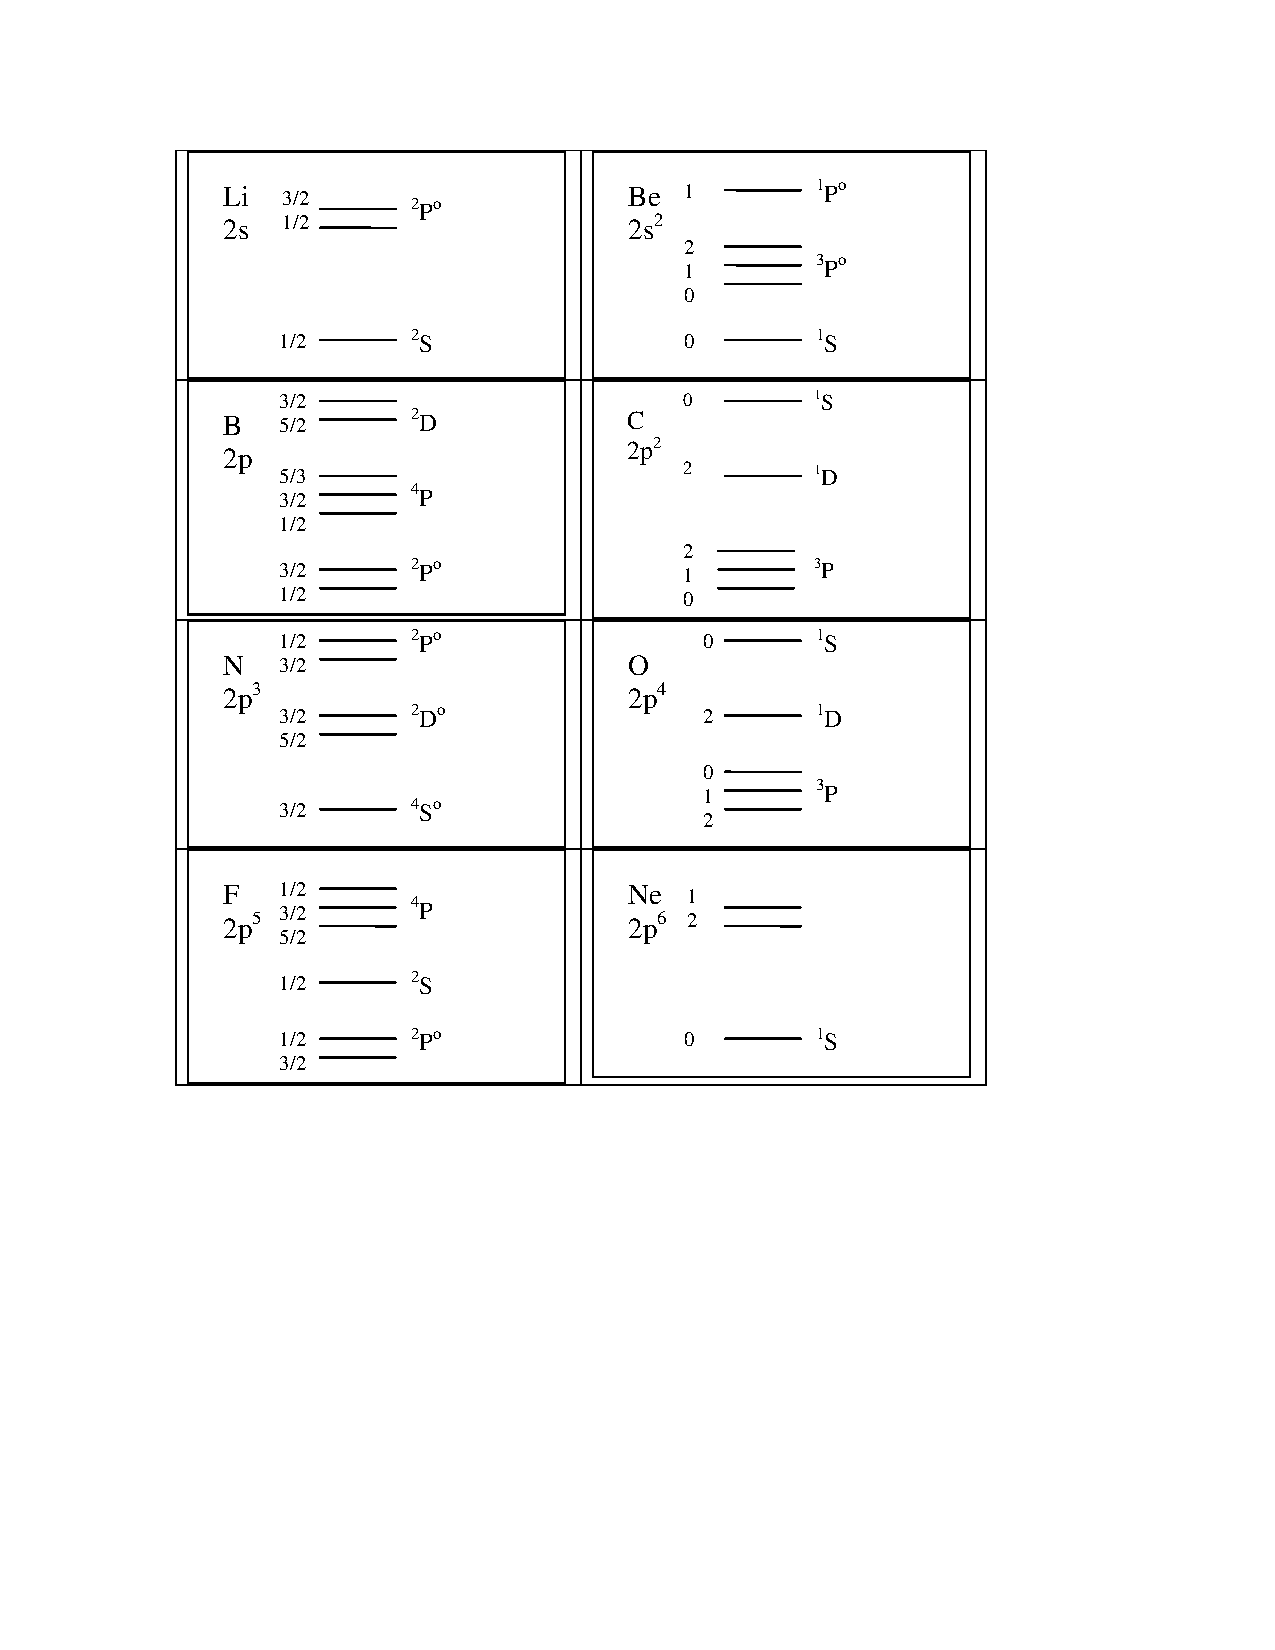
\includegraphics{EnergyLevelsSecondRow}
\caption[Energy level diagrams for second-row elements]{Energy-level diagrams for the second row isoelectronic
sequences. The levels are correct for first ion and higher, but may not
be for some atoms, or for ions of elements with more mass than~K.}
\label{fig:EnergyLevelsSecondRow}
\end{figure}

Table \ref{tab:IsoSequences} lists all isoelectronic sequences for the first thirty elements.
The bottom row on the table indicates the shell number, in the nomenclature
used for the photoionization shell layering\footnote{The arrays within the code count on the C scale so start from 0 and are one less than the index shown in the table.}.
A superscript ``1'' indicates that the atom or first ion has a non-standard configuration in the outer shell.

\begin{table}
\label{tab:IsoSequences}
\caption{Isoelectronic Sequences}
\begin{tabular}{llllllllll}
\hline
1 H&   2 He&  3 Li&  4 Be&  5 B&  6 C&  7 N&  8 O&  9 F&  10 Ne\\
\hline
1s $^2$S& 1s$^2$ $^1$S& 2s$^2$S& 2s$^2$ $^1$S& 2p $^2$P& 2p$^2$ $^3$P&
2p$^3$ $^4$S& 2p$^4$ $^3$P& 2p$^5$ $^2$P& 2p$^6$ $^1$S\\
H 1& He 1& Li 1& Be 1& Bo 1& C 1& N 1& O 1& F 1& Ne 1\\
He 2& Li 2& Be 2& Bo 2& C 2& N 2& O 2& F 2& Ne 2& Na 2\\
Li 3& Be 3& Bo 3& C 3& N 3& O
3& F 3& Ne 3& Na 3& Mg 3\\
Be 4& Bo 4& C 4& N 4& O 4& F 4& Ne 4& Na 4& Mg 4& Al 4\\
Bo 5& C 5& N 5& O
5& F 5& Ne 5& Na 5& Mg 5& Al 5& Si 5\\
C 6& N 6& O 6& F 6& Ne 6& Na 6& Mg 6& Al 6& Si 6& P 6\\
N 7& O 7& F 7& Ne 7& Na 7& Mg 7& Al 7& Si 7& P 7& S 7\\
O 8& F  8& Ne 8& Na 8& Mg 8& Al 8& Si 8& P  8& S  8&Cl 8\\
F 9& Ne 9& Na 9& Mg 9& Al 9& Si 9& P  9& S 9& Cl 9& Ar 9\\
 Ne10& Na10&Mg10& Al10& Si10& P 10& S
10& Cl10& Ar10& K 10\\
Na11& Mg11& Al11& Si11& P 11& S 11& Cl11& Ar11& K 11& Ca11\\
 Mg12& Al12&
Si12& P 12& S
12& Cl12& Ar12& K 12& Ca12& Sc12\\
Al13& Si13& P 13& S 13& Cl13& Ar13& K 13& Ca13& Sc13& Ti13\\
Si14& P 14&
S 14& Cl14& Ar14& K 14& Ca14& Sc14& Ti14& V 14\\
P 15& S 15& Cl15& Ar15& K 15& Ca15& Sc15& Ti15& V 15& Cr15\\
S 16& Cl16& Ar16& K 16& Ca16& Sc16& Ti16& V 16& Cr16& Mm16\\
Cl17& Ar17&K 17& Ca17& Sc17& Ti17& V 17& Cr17& Mm17& Fe17\\
Ar18& K 18& Ca18& Sc18& Ti18& V 18& Cr18& Mm18& Fe18& Co18\\
K 19& Ca19& Sc19& Ti19& V
19& Cr19& Mm19& Fe19& Co19& Ni19\\
Ca20& Sc20& Ti20& V 20& Cr20& Mm20& Fe20& Co20& Ni20& Cu 20\\
Sc21& Ti21& V
21& Cr21& Mm21& Fe21& Co21& Ni21& Cu 21& Zn 21\\
Ti22& V 22& Cr22& Mm22& Fe22& Co22& Ni22& Cu 22& Zn 22\\
V 23& Cr23& Mm23& Fe23& Co23& Ni23& Cu 23& Zn 23\\
Cr24& Mm24& Fe24& Co24& Ni24& Cu 24& Zn 24\\
Mm25& Fe25& Co25& Ni25& Cu 25& Zn 25\\
Fe26& Co26& Ni26& Cu 26& Zn 26\\
Co27& Ni27& Cu 27& Zn 27\\
Ni28& Cu 28& Zn 28\\
Cu 29& Zn 29\\
Zn 30\\
1&1&2&2&3&3&3&3&3&3\\
\hline
\end{tabular}
\end{table}

\begin{tabular}{llllllllll}
\hline
11 Na&  12 Mg&  13 Al&  14 Si&  15 P&   16 S&   17 Cl&  18 Ar&  19 K&   20
Ca\\
\hline
3s $^2$S& 3s$^2$ $^1$S& 3p $^2$P& 3p$^2$ $^3$P& 3p$^3$ $^4$S& 3p$^4$ $^3$P&
3p$^5$ $^2$P& 3p$^6$ $^1$S& 3d $^2$D& 3d$^2$ $^3$F\\
Na 1& Mg 1& Al 1& Si 1& P
1& S  1& Cl 1& Ar 1& K  1$^1$ & Ca 1$^1$\\
Mg 2& Al 2& Si 2& P  2& S  2& Cl 2& Ar 2& K  2& Ca 2$^1$& Sc 2$^1$\\
Al 3& Si
3& P 3& S  3& Cl 3& Ar 3& K  3& Ca 3& Sc 3& Ti 3\\
Si 4& P 4& S  4& Cl 4& Ar 4& K  4& Ca 4& Sc 4& Ti 4& V 4\\
P 5& S  5& Cl 5& Ar 5& K  5& Ca 5& Sc 5& Ti 5& V  5& Cr 5\\
S  6& Cl 6& Ar 6& K  6& Ca 6& Sc 6& Ti 6& V
6& Cr 6& Mm 6\\
Cl 7& Ar 7& K  7& Ca 7& Sc 7& Ti 7& V  7& Cr 7& Mm 7& Fe 7\\
Ar 8& K  8& Ca 8& Sc 8& Ti 8& V
8& Cr 8& Mm 8& Fe 8& Co 8\\
K  9& Ca 9& Sc 9& Ti 9& V  9& Cr 9& Mm 9& Fe 9& Co 9& Ni 9\\
Ca10& Sc10& Ti10& V
10& Cr10& Mm10& Fe10& Co10& Ni10& Cu 10\\
 Sc11& Ti11& V 11& Cr11& Mm11& Fe11& Co11& Ni11& Cu 11& Zn 11\\
 Ti12& V
12& Cr12& Mm12& Fe12& Co12& Ni12& Cu 12& Zn 12\\
V 13& Cr13& Mm13& Fe13& Co13& Ni13& Cu 13& Zn
13\\
Cr14& Mm14& Fe14& Co14& Ni14& Cu 14& Zn 14\\
 Mm15& Fe15& Co15& Ni15& Cu 15& Zn 15\\
Fe16& Co16& Ni16& Cu
16& Zn 16\\
Co17& Ni17& Cu 17&  Zn 17\\
Ni18& Cu 18&  Zn 18\\
Cu 19& Zn 19\\
Zn 20\\
4& 4&5&5&5&5&5&5&6&6\\
\hline
\end{tabular}

\begin{tabular}{lllllllllll}
\hline
21 Sc&  22 Ti&  23 V&   24 Cr&  25 Mm&  26 Fe&  27 Co&  28 Ni&  29 Cu& 30
Zn\\
\hline
3d$^3$ $^4$F& 3d$^4$
$^5$D& 3d$^5$ $^6$S& 3d$^6$ $^5$D& 3d$^7$ $^4$F& 3d$^8$ $^3$F& 3d$^9$ $^2$D&
3d$^{10}$ $^1$S& 4s $^2$S& 4s$^2$ $^1$S\\
Sc 1& Ti 1& V  1& Cr 1& Mm 1& Fe
1& Co 1& Ni 1& Cu 1& Zn 1\\
Ti 2& V 2& Cr 2& Mm 2& Fe 2& Co 2& Ni 2& Cu 2& Zn 2\\
V  3& Cr 3& Mm 3& Fe 3& Co
3& Ni 3& Cu 3& Zn 3\\
Cr 4& Mm 4& Fe 4& Co 4& Ni 4& Cu 4& Zn 4\\
Mm 5& Fe 5& Co 5& Ni 5& Cu 5& Zn 5\\
Fe 6& Co
6& Ni 6& Cu 6& Zn 6\\
Co 7& Ni 7& Cu 7& Zn 7\\
Ni 8& Cu 8& Zn 8\\
Cu 9& Zn 9\\
Zn 10\\
6&6&6&6&6&6&6&6&7&7\\
\hline
\end{tabular}

\section{Be-sequence}

The model atom used for Be-like ions (C~III, N~IV, O~V, Al~II, Si~III, S~IV,
etc) is shown in Figure~\ref{fig:BeSequenceEnergyLevels}.

\begin{figure}
\centering
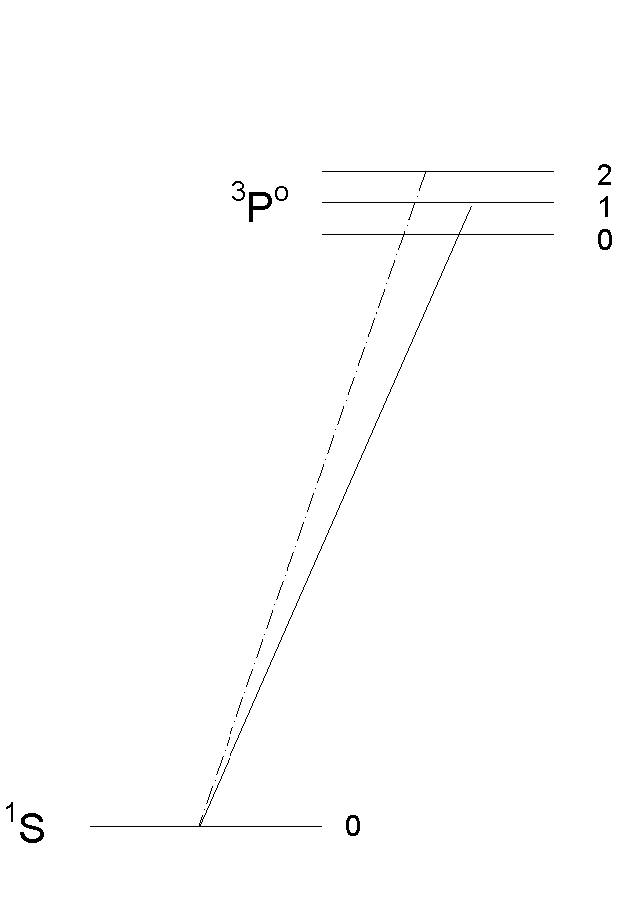
\includegraphics[scale=0.6]{BeSequenceEnergyLevels}
\caption[Be-sequence model atom]{The Be-sequence model atom.  The permitted transition is marked
``UV1,'' while the forbidden and intercombination transitions are ``For''
and ``Int.''}
\label{fig:BeSequenceEnergyLevels}
\end{figure}

\section{Carbon}

\dots

\section{Nitrogen}

Photoionization from the excited $^2D$
level of $N^0$ is included, and can be the dominant ionization mechanism in
well-shielded regions.\footnote{Neutral and first ion have non-standard filling.}

\section{Oxygen}

Photoionization from the first two excited states of O$^{2+}$ is included
as a general ionization mechanism.  This can dominate the ionization of
the ion since it occurs behind the He$^+$ - He$^{++}$ ionization front, which shields
the region from 4 Ryd and higher radiation.   Similarly, photoionization
from the first excited state and all inner shells of $O^0$ are included.

\subsection{The O I model atom}

A partial Grotrian diagram for the O I atom considered in the L$\beta$-O I
fluorescence problem is shown in Figure \ref{fig:OI_EnergyLevels}.  Multiplet averaged transition
probabilities are taken from unpublished Opacity Project data, and the
collision strengths are from the $\bar g$
 approximation for collisions between electrons and neutrals.  Rates
for fluorescence between the two transitions are computed as in
\citet{Netzer1985}.

\begin{figure}
\centering
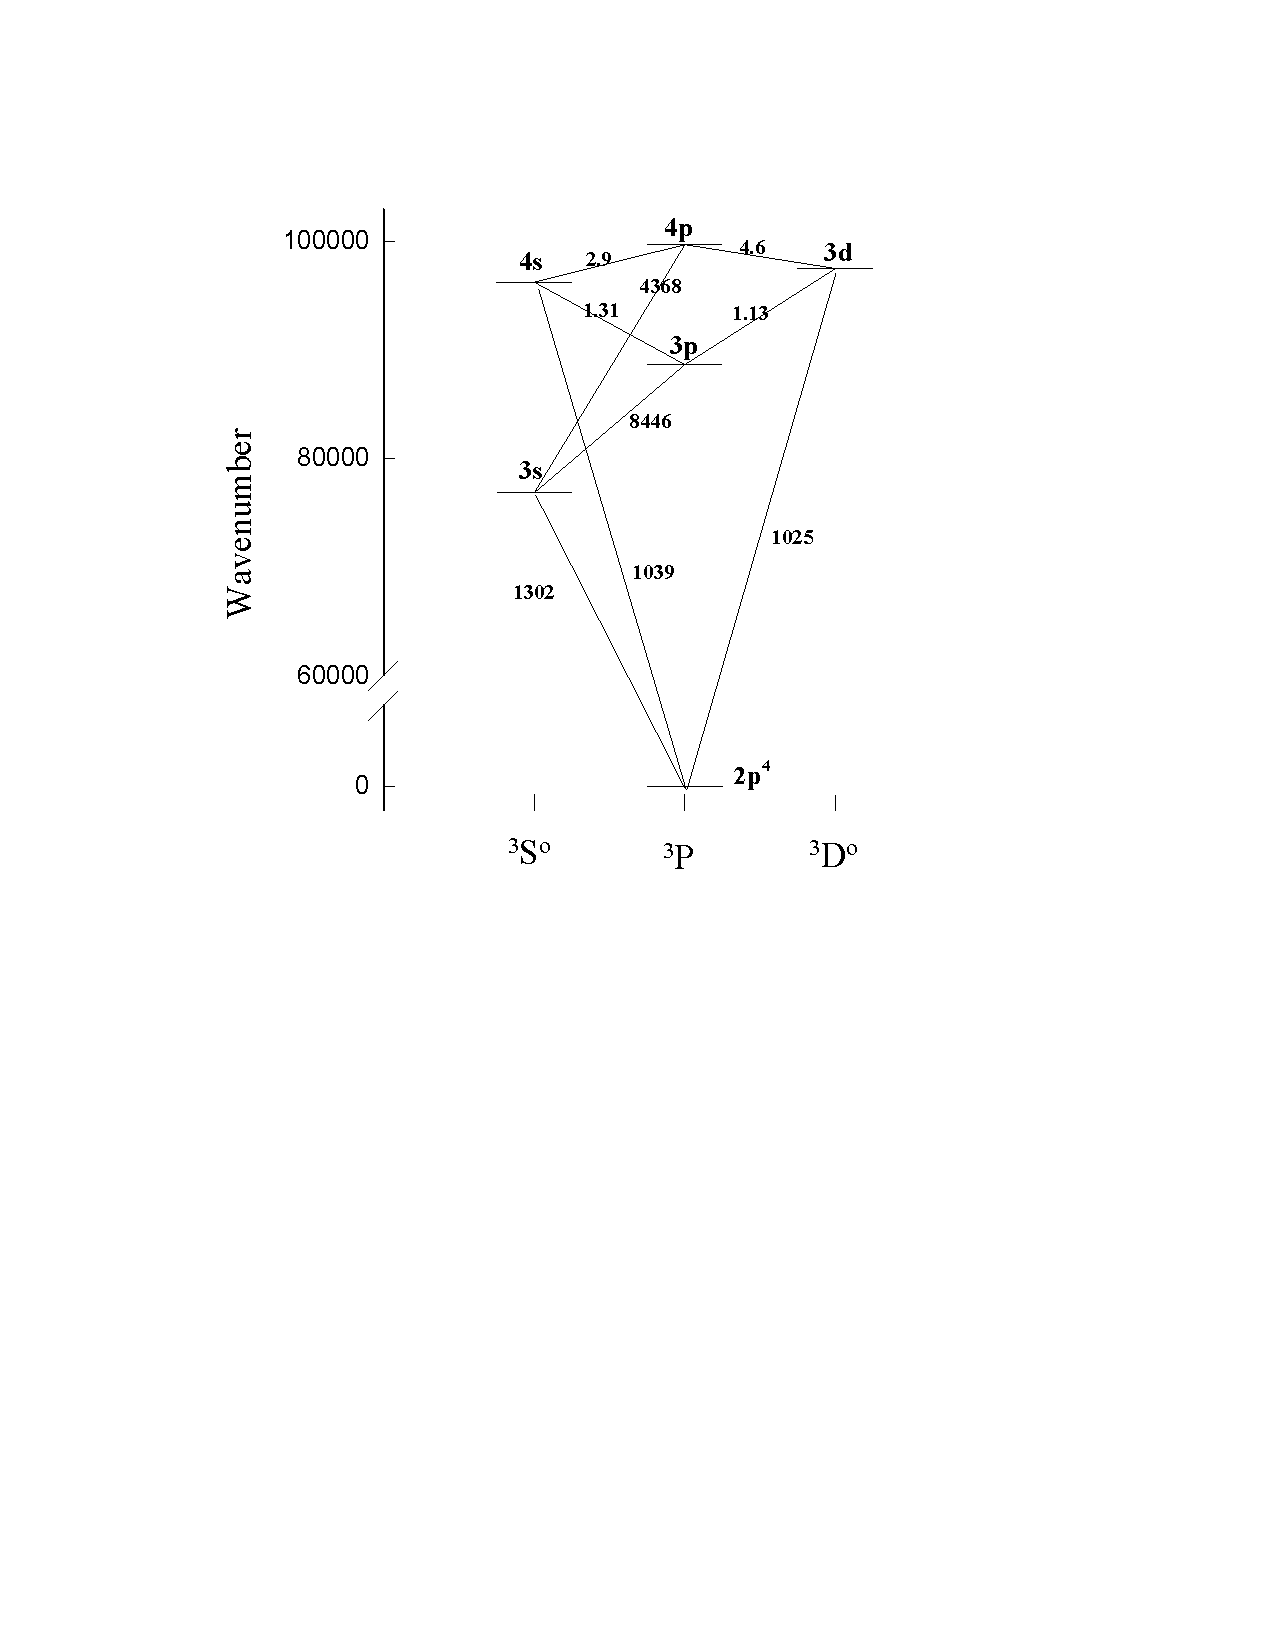
\includegraphics[scale=0.8]{OI_EnergyLevels}
\caption[O~I energy levels]{The levels of O$^o$ included in the calculation of the
OI-L$_{\beta}$ pumping
problem are shown.}
\label{fig:OI_EnergyLevels}
\end{figure}

\section{Neon}


\section{Magnesium}

Photoionization from the excited $^2P^0$ level of $Mg^+$ is included as a general
$Mg^+$ destruction mechanism using Opacity Project data retrieved from
\cdTerm{TOPBase}.
This can easily be the dominant Mg$^+$ destruction mechanism in
dense gas
since the excited state has an ionization potential below 1 Ryd.  The code
will generate a comment at the end of the calculation if this is a
competitive $Mg^+$ destruction mechanism.

\section{Aluminum}


\section{Calcium}

The Ca II ion is treated as a five-level atom plus continuum.  The model
atom is shown in Figure \ref{fig:CaIIEnergyLevels}, and is similar to that described by \citet{Shine1974}.  Collision strengths for j-mixing collisions are from \citet{Saraph1970}.  Collision and radiative data for the $4s - 4p$ transition are taken
from the compendium of \citet{Mendoza1983}, and all other collision data are
from \citet{Chidichimo1981} and \citet{Saraph1970}.  Radiative data for the $3d - 4p$
and $4s - 3d$ transitions are from
\citet{BlackWeisheit1972}; these
are in good agreement with the calculations of \citet{Osterbrock1951}.  The
compendium by \citet{Shine1974} provides photoionization cross sections
for excited levels, which are adopted here.  Photoionization of the excited
$^2D$ level by \la\ (\citealp{Wyse1941}) and all other line or continuum sources is
explicitly included.  Recombination contributions to the population of
individual levels are included by dividing the excited state recombination
coefficient among the excited levels considered, according to their
statistical weight and the rules of LS coupling.

\begin{figure}
\centering
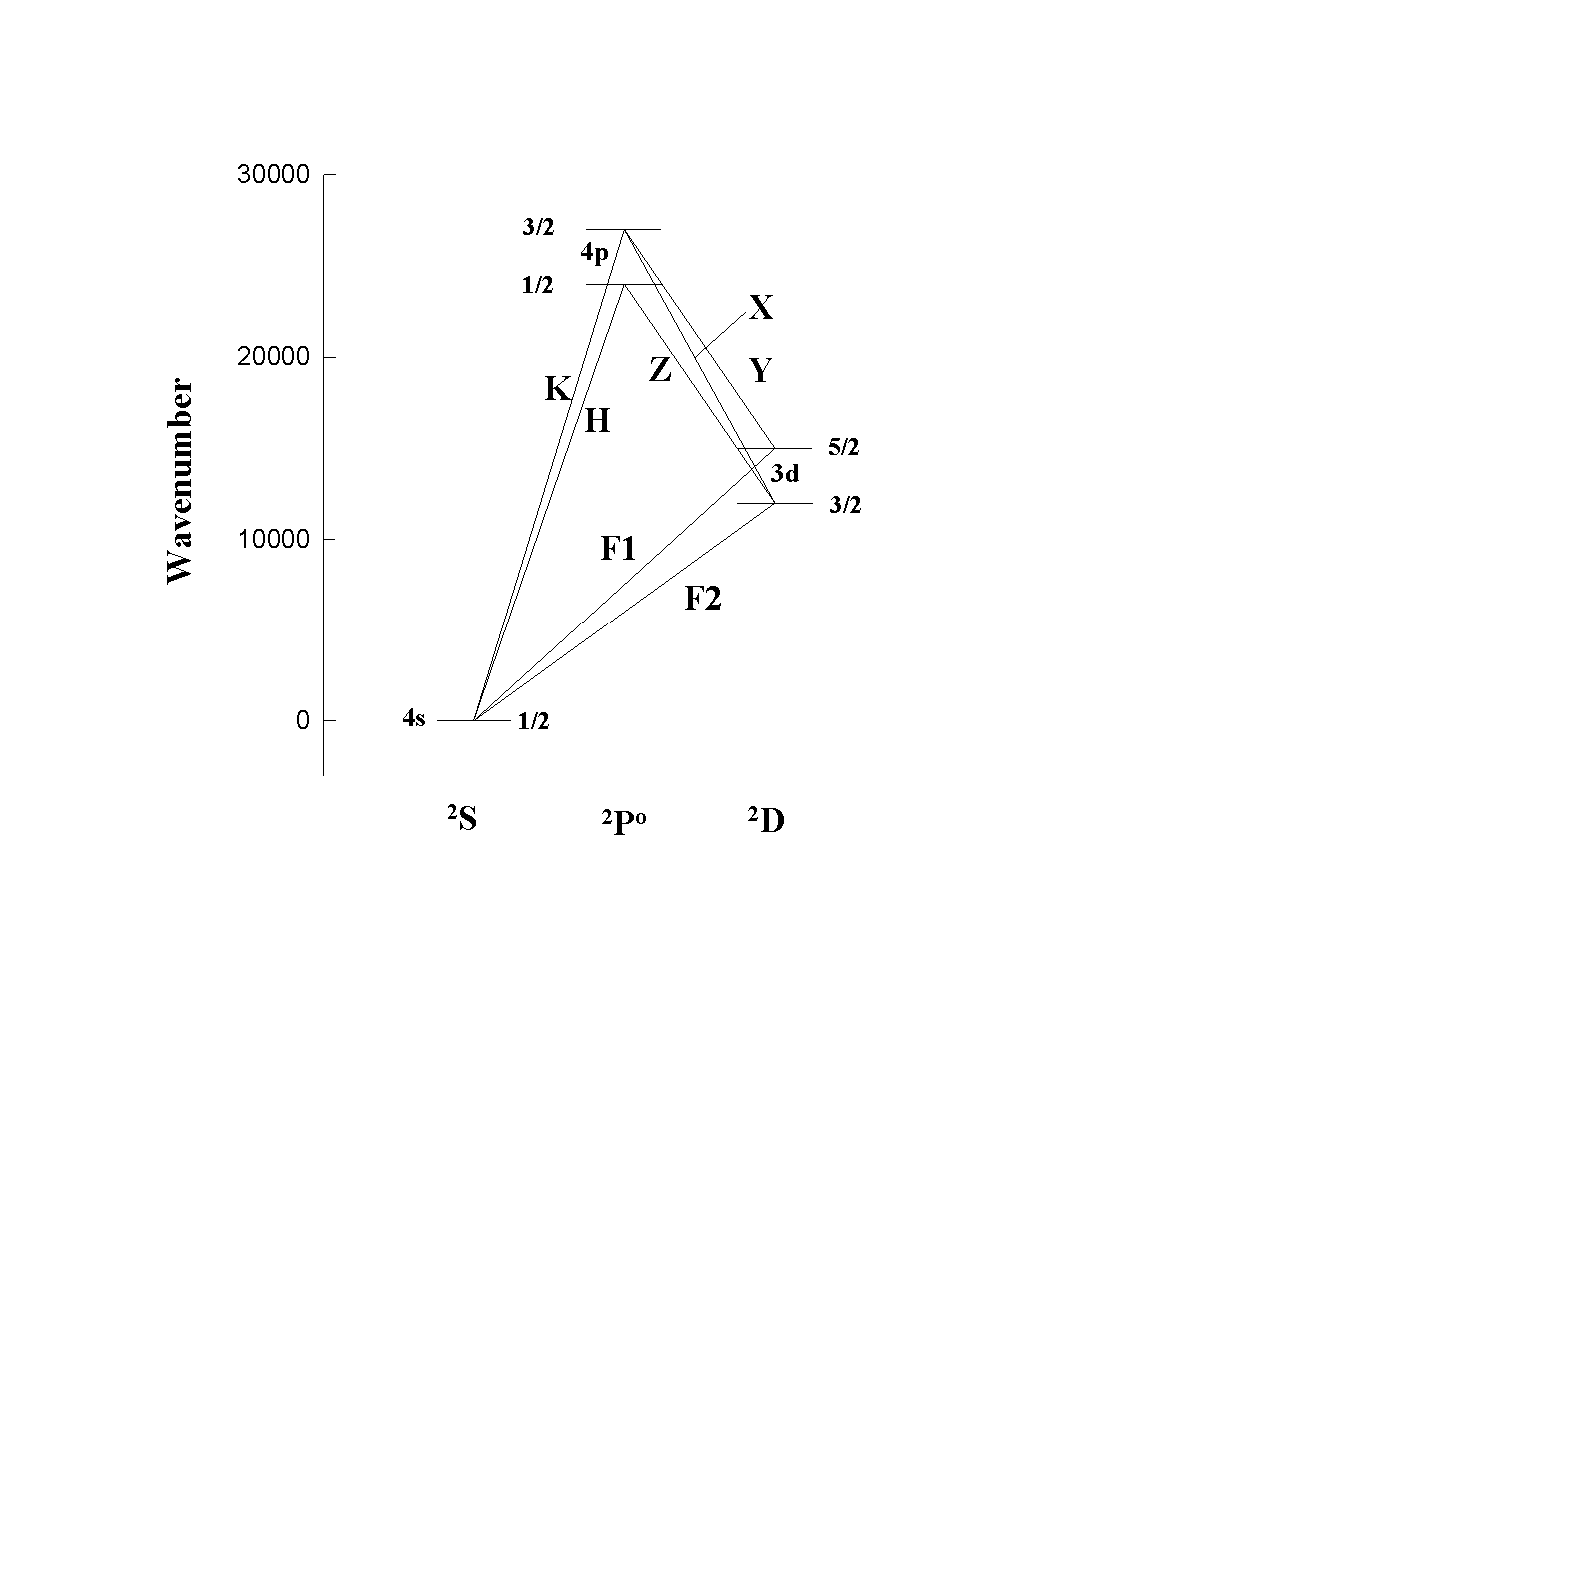
\includegraphics[scale=0.7]{CaIIEnergyLevels}
\caption[CaII model atom]{The five levels of Ca$^+$ included in the calculations are shown.
The wavelengths of the predicted lines are K (3934), H (3969), X (8498),
Y (8542), Z (8662), F1 (7291), and F2 (7324).}
\label{fig:CaIIEnergyLevels}
\end{figure}

All Ca~II transitions (including the forbidden lines) can become quite
optically thick.  Radiative transfer is treated with the escape probability
formalism, assuming incomplete redistribution, including destruction by
background opacities.

\section{Iron}

Low temperature dielectronic recombination rate coefficients have not
been computed for this element.  Means of first-ion rtes are used.  Charge transfer
rate coefficients are from \citet{Neufeld1989} and
\citet{Ferland1997}.

The \feii\ ion is described by \citet{Verner1999} and in sections of
Part I of this document.  In the current implementation up to 376 levels
can be included. This is an area of extensive activity.
Figure \ref{fig:FeII_model} shows
the lowest 16 levels of the atom and some of the lines predicted.

\begin{figure}
\centering
\label{fig:FeII_model}
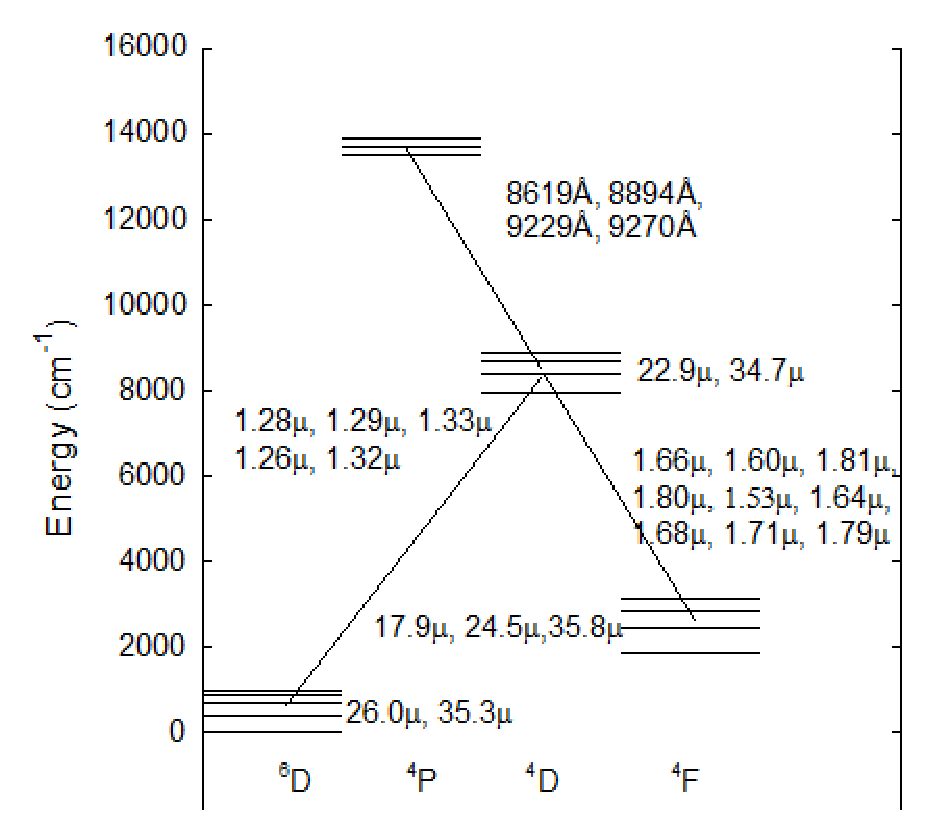
\includegraphics[scale=0.7]{FeII_model}
\caption[\feii\ model of low-lying levels]{The sixteen level atom used to compute \feii\ IR emission.  Lines
predicted are indicated.}
\end{figure}

Fe~IV is treated as a twelve-level atom, with energies from
\citet{Sugar1985}, transition probabilities from \citet{Garstang1958}, and collision
strengths from \citet{Berrington1995}.
Figure \ref{fig:FeIV_model} shows the model atoms
with the lines predicted by the code indicated.

\begin{figure}
\centering
\label{fig:FeIV_model}
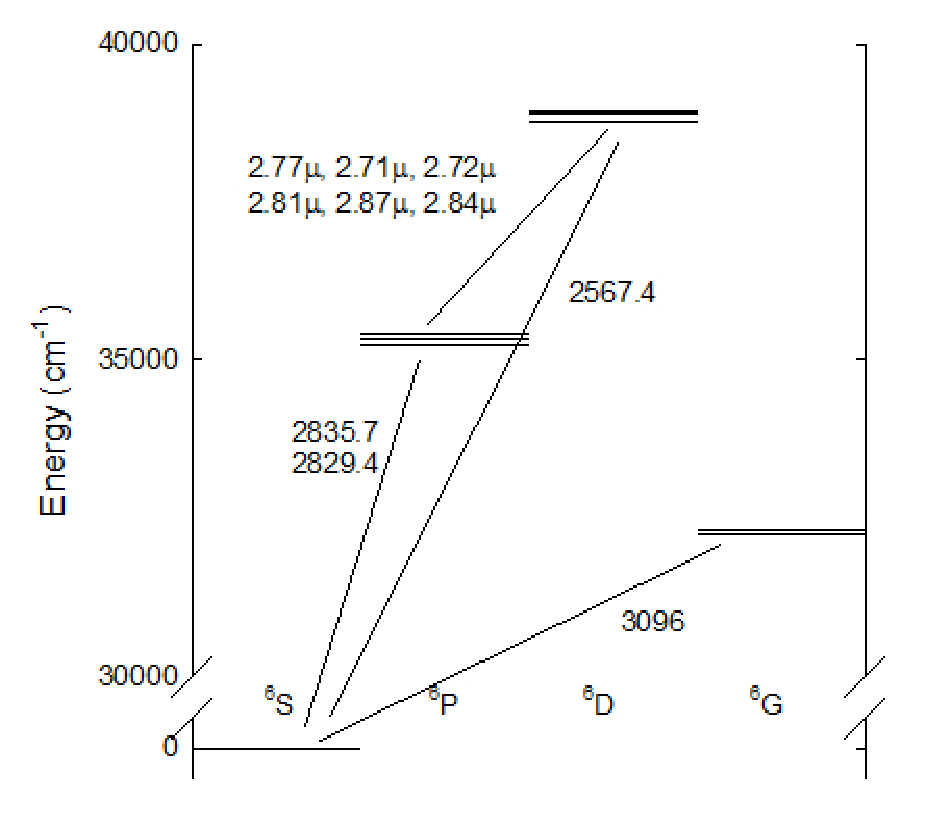
\includegraphics[scale=0.8]{FeIV_model}
\caption[Fe~IV model atom]{The twelve level atom used to compute Fe~IV emission.  Lines
predicted are indicated.}
\end{figure}

Fe~VII is treated as an eight-level system.
Figure \ref{fig:Fe7_levels} shows the levels
and stronger emission lines.
Atomic data are from \citet{Berrington2000}.

\begin{figure}
\centering
\label{fig:Fe7_levels}
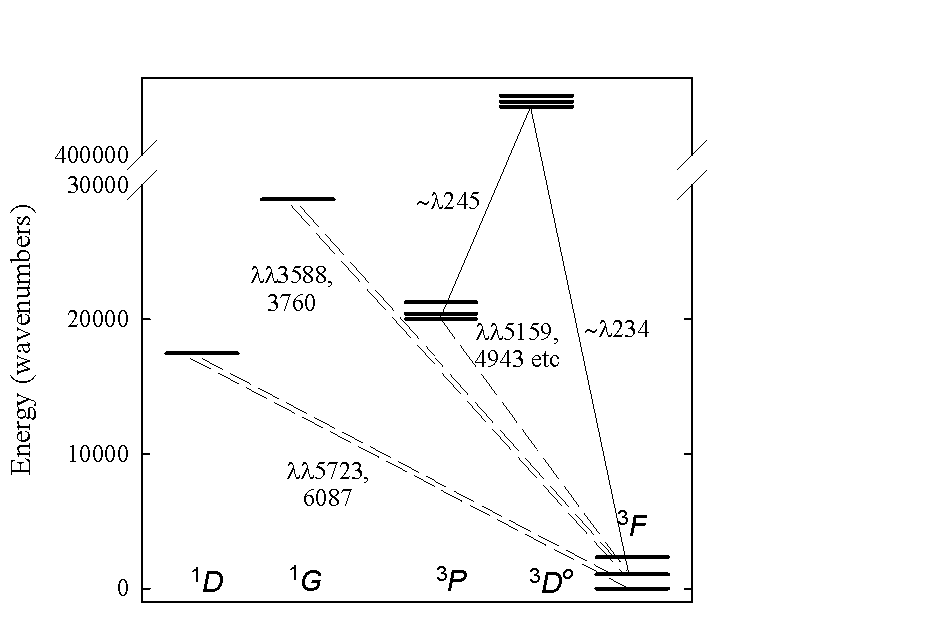
\includegraphics[scale=0.9]{Fe7_levels}
\caption[Fe~VII model atom]{The eight-level atom used to compute Fe~VII emission.  Lines
predicted are indicated.}
\end{figure}

\subsection{Fe K$\alpha$ emission}

The intensity of the Fe~K$\alpha$ line is predicted including both recombination
and fluorescence.  Figure \ref{fig:FeKalpha} shows the fluorescence yield and
K$\alpha$ energy.
The line predictions are separated into ``cold'' iron (i.e., iron with
M-shell electrons present) and ``hot'' iron (those ionization states
producing lines with energies greater than $\sim$6.4 keV).  This includes the
recombination and collisional contribution.  The ``TOTL'' K$\alpha$ is the sum of
the two.

\begin{figure}
\centering
\label{fig:FeKalpha}
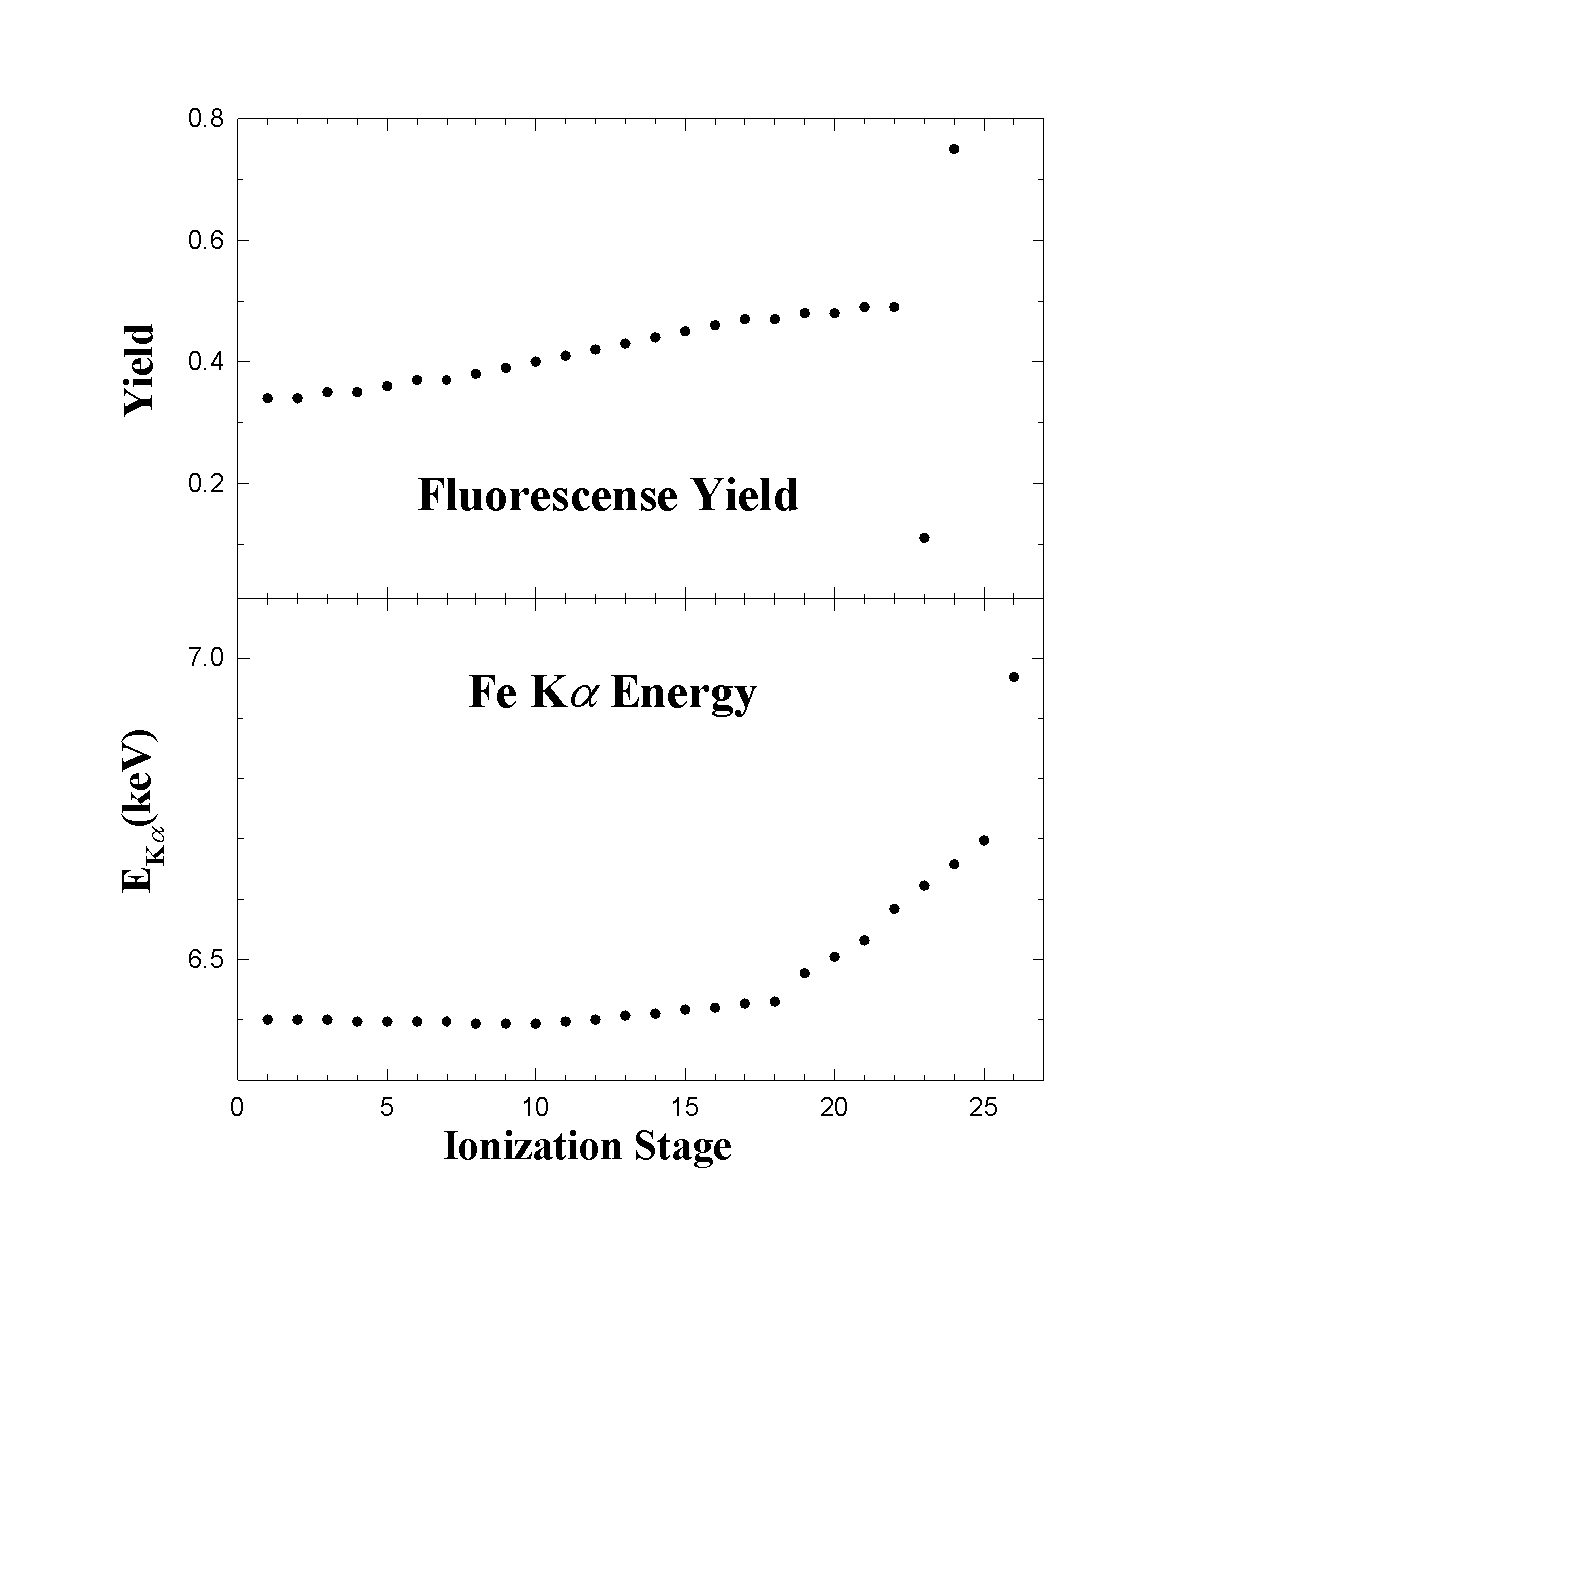
\includegraphics[scale=0.8]{FeKalpha}
\caption[Fe~K$\alpha$ yield and energy]{The fluorescence yield and energy of the emitted Fe~K$\alpha$ photon
are shown as a function of ionization stage.}
\end{figure}

\section{Heavy element opacities}

Figure \ref{fig:GasOpacity} shows a calculation of the opacity of a solar gas with very
low ionization.

\begin{figure}
\centering
\label{fig:GasOpacity}
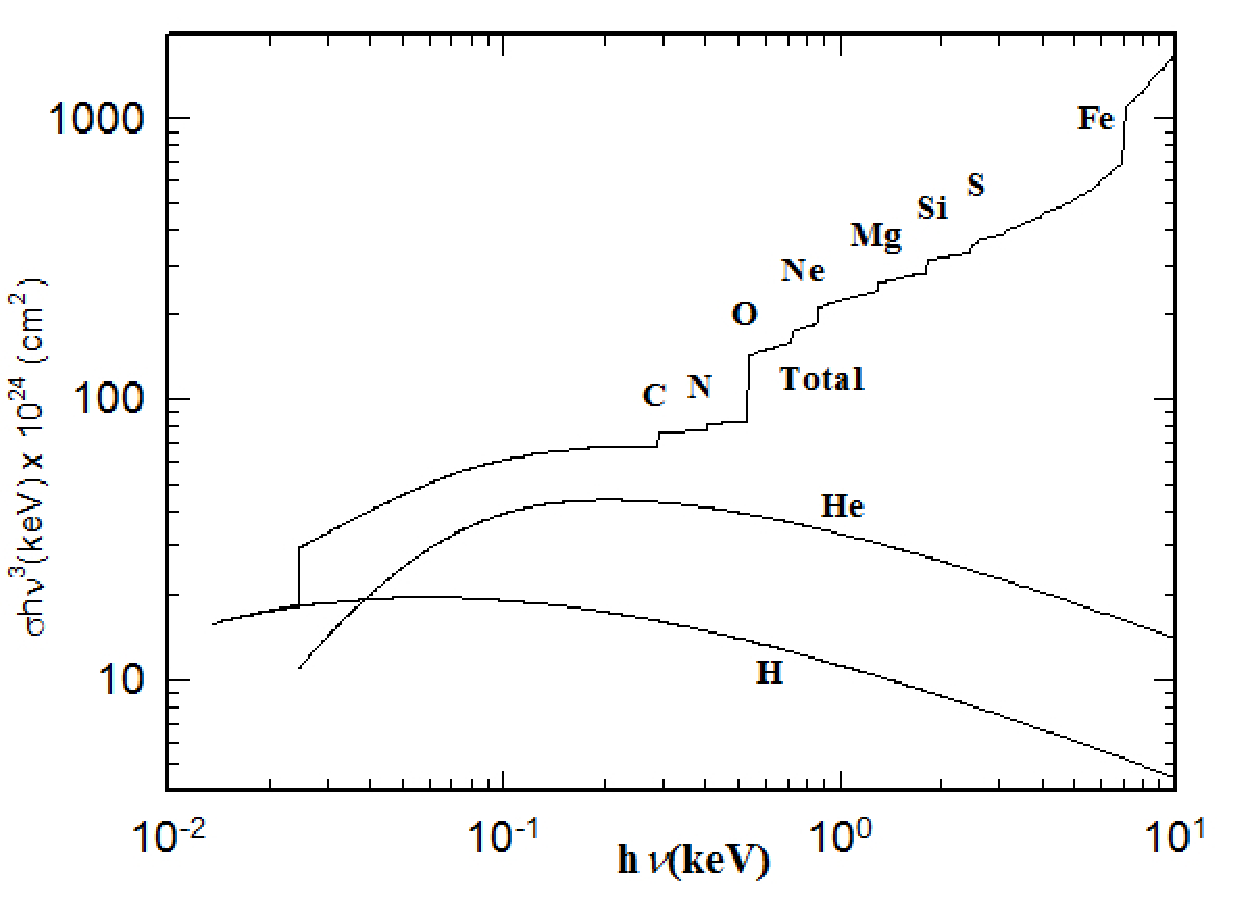
\includegraphics[scale=0.7]{GasOpacity}
\caption[Atomic gas opacity]{The opacity of a neutral gas with solar abundances is shown
as a function of energy.  The curve is scaled to allow direct comparison
with conventional calculations of opacity at X-Ray energies (i.e., \citet{Morrison1983}. hevopc}
\end{figure}

\section{Overall reliability}

It is difficult to estimate the overall uncertainty present in an
ionization balance calculation.  The current photoionization cross-section
data are based on accurate experiments or the Opacity Project (\citealp{VernerFerlandKorista1996}).  These should be accurate to roughly 10\% except near resonances.
Although resonances are included in the Opacity Project data, the positions
of these resonances are uncertain by more than their width because the OP
was not intended as an atomic structure calculation.  Recombination
coefficients including low temperature dielectronic recombination have yet
to be computed for the majority of the stages of ionization of the elements
now in \Cloudy, but recombination from parent ions with closed shells is
not affected, and good rates exist \citep{VernerFerland1996}.

It is possible to make a subjective estimate of the uncertainty in the
calculation of the ionization balance for nebular temperatures.
Table~\ref{tab:IonizationBalanceReliability}
lists the elements now included in the calculations and gives this estimate
of the uncertainty.  For recombination from a closed shell autoionization
resonances do not occur near threshold, recombination is primarily radiative,
and the calculations should be virtually exact.  Dielectronic recombination
rates are also known for those species treated by
Nussbaumer and Storey.
These are given a quality weighting of~A.

\begin{table}
\caption{Ionization Balance Reliability}
\label{tab:IonizationBalanceReliability}
\begin{tabular}{lllllllllll}
\hline
1& H&2 He&3 Li&4 Be&5 B&6 C&7 N&8 O&9 F&10 Ne\\
\hline
1&A&A&A&B&B&B&B&B&B&B\\
2&& A&A&A&B&B&B&B&B&B\\
3&&&A&A&A&B&B&B&B&B\\
4&&&&A&A&A&B&B&B&B\\
5&&&&&A&A&A&B&B&B\\
6&&&&&&A&A&A&B&B\\
7&&&&&&&A&A&A&B\\
8&&&&&&&&A&A&A\\
9&&&&&&&&&A&A\\
10&&&&&&&&&&A\\
\hline
\end{tabular}
\end{table}


\begin{table}
\caption{Ionization Balance Reliability Continued}
\begin{tabular}{lllllllllllll}
\hline
&11 Na&12 Mg&13 Al&14 Si&15 P&16 S&17 Cl&18 Ar&19 K&20 Ca\\
\hline
1&B&B\\
2&B&B&B\\
3&B&B&B&B\\
4&B&B&B&B&B\\
5&B&B&B&B&B&B\\
6&B&B&B&B&B&B&B\\
7&B&B&B&B&B&B&B&B\\
8&B&B&B&B&B&B&B&B&B\\
9&A&B&B&B&B&B&B&B&b&B\\
10&A&A&B&B&B&B&B&B&B&B\\
11&A&A&A&B&B&B&B&B&B&B\\
12&&A&A&A&B&B&B&B&B&B\\
13&&&A&A&A&B&B&B&B&B\\
14&&&&A&A&A&B&B&B&B\\
15&&&&&A&A&A&B&B&B\\
16&&&&&&A&A&A&B&B\\
17&&&&&&&A&A&A&B\\
18&&&&&&&&A&A&A\\
19&&&&&&&&&A&A\\
20&&&&&&&&&&A\\
\hline
\end{tabular}
\end{table}

\begin{table}
\caption{Ionization Balance Reliability Continued}
\begin{tabular}{lllllllllllll}
\hline
&21 Sc&22 Ti&23 V&24 Cr&25 Mn&26 Fe&27 Co&28 Ni&29 Cu&30
Zn&\\
1\\
2\\
3\\
4\\
5\\
6\\
7\\
8\\
9\\
10&B\\
11&B&B\\
12&B&B&B&\\
13&B&B&B&B\\
14&B&B&B&B&B\\
15&B&B&B&B&B&B\\
16&B&B&B&B&B&B&B\\
17&B&B&B&B&B&B&B&B\\
18&B&B&B&B&B&B&B&B&B\\
19&A&B&B&B&B&B&B&B&B&B\\
20&A&A&B&B&B&B&B&B&B&B\\
21&A&A&A&B&B&B&B&B&B&B\\
22&&A&A&A&A&B&B&B&B&B\\
23&&&A&A&A&B&B&B&B&B\\
24&&&&A&A&A&B&B&B&B\\
25&&&&&A&A&A&B&B&B\\
26&&&&&&A&A&A&B&B\\
27&&&&&&&A&A&A&B\\
28&&&&&&&&A&A&A\\
29&&&&&&&&&A&A\\
30&&&&&&&&&&A\\
\hline
\end{tabular}
\end{table}

These uncertainties refer to the ionization balance of an optically thin
cell of gas at nebular temperatures.  The intensities of emission lines
will be less uncertain than this for two reasons. First, the thermostat
effect of any collisionally excited line prevents its intensity from changing
by much.  Second is the fact that the integrated column density in an ion
is affected as much by (fairly exact) quantities such as the ionization
structure of H or He, as by the atomic data of a particular ion.  At coronal
temperatures the Burgess mechanism dominates, and the situation should be
somewhat better.

Nigel Badnell and collaborators have begun a program to compute
dielectronic recombination rate coefficients along isoelectronic sequences.
These have appeared in a series of papers in A\&A starting in 2003.  Ions
which have been done by Badnell et al. appear as B in the table.  They have
not yet produced radiative recombination rates.

\section{Solving the ionization ladder }

   The rate of change of the density of a particular ionization state i
is given by
\begin{equation}
\frac{{\partial {n_i}}}{{\partial t}} = {G_i} + \sum\limits_{j \ne i}
{{R_{j \to i}}{n_j}}  - {n_i}\left( {{L_i} + \sum\limits_{j \ne i} {{R_{i
\to j}}} } \right)\quad
[\mathrm{cm}^{-3} \mathrm{s}^{-1}].% (1)
\end{equation}
Gains $G_i$ [cm$^{-3}$~s$^{-1}$] and losses $L_i$~[s$^{-1}$] represent physical processes that
remove atoms from the ionization ladder.  Advection, or molecular processes
that create or destroy atoms and ions, are examples.  The terms $R_{nm}$ are
rates (s$^{-1}$) for processes that move atoms up or down the ionization ladder.

Several physical processes strongly couple
non-adjacent stages of ionization.  Charge transfer on grain surfaces and
advection are examples.  The full system of equations is solved using standard
linear algebra methods.

\section{Ionization potentials of subshells}

Table \ref{tab:SubshellIonizationPotentials} gives ionization potentials
of the subshells.

\begin{table}
\label{tab:SubshellIonizationPotentials}
\caption{Ionization Potentials of Subshells (eV)}
\begin{tabular}{lllllllllll}
\hline
Element\\
\hline
H&    1\\
\hline
1s& 13.60\\
\hline
He&   1&   2\\
\hline
1s& 24.59& 54.42\\
\hline
Li&   1&   2&   3\\
\hline
1s& 64.39& 75.64& 122.5\\
2s& 5.392\\
\hline
Be&   1&   2&   3&   4\\
\hline
1s& 119.3& 129.9& 153.9& 217.7\\
2s& 9.323& 18.21\\
\hline
B& 1&   2&   3&   4&   5\\
\hline
1s& 194.0& 209.8& 227.4& 259.4& 340.2\\
2s& 14.05& 25.16& 37.93\\
2p& 8.298\\
\hline
C&    1&   2&   3&   4&   5&   6\\
\hline
1s& 291.0& 307.6& 328.9& 352.2& 392.1& 490.0\\
2s& 19.39& 30.47& 47.89& 64.49\\
2p& 11.26& 24.38\\
\hline
N&    1&   2&   3&   4&   5&   67   7\\
\hline
1s& 404.8&
423.6& 447.3& 475.3& 504.3& 552.1& 667.1\\
2s& 25.41& 37.96& 55.45& 77.47& 97.89\\
2p& 14.53&
29.60& 47.45\\
\hline
O& 1& 2& 3& 4& 5& 6& 7& 8\\
\hline
1s& 538.0& 558.1& 584.0& 614.4&
649.1& 683.7& 739.3& 871.4\\
2s& 28.48& 45.99& 65.51& 87.37& 113.9& 138.1\\
2p& 13.62& 35.12&
54.94& 77.41\\
\hline
F&    1&   2&   3&   4&   5&   6&   7&   8&   9\\
\hline
1s& 694.0& 712.2& 739.2& 770.9&
809.1& 850.2& 890.5& 953.9&  1103\\
2s& 37.86& 54.59& 76.10& 99.57& 126.2& 157.2& 185.2\\
2p& 17.42& 34.97& 62.71& 87.14& 114.2\\
\hline
\end{tabular}
\end{table}

\begin{table}
\caption{Ionization Potentials of Subshells (eV) continued}
\begin{tabular}{lllllllllll}
\hline
Ne&   1&   2&   3&   4&   5&   6&   7&   8&   9&  10\\
1s& 870.1& 883.1& 913.1& 948.0& 987.3&
1031&  1078&  1125&  1196&  1362\\
2s& 48.47& 63.74& 87.21& 113.2& 141.5& 171.9& 207.3&
239.1\\
2p& 21.56& 40.96& 63.46& 97.12& 126.2& 157.9\\
\hline
Na&   1&   2&   3&   4&   5&   6&
7&   8&   9&  10\\
\hline
1s&  1079&  1097&  1118&  1143&  1185&  1230&  1281&  1335&  1386&  1465\\
2s&
70.84& 73.47& 99.45& 126.9& 156.7& 189.9& 224.4& 264.2& 299.9\\
2p& 38.14& 47.29& 71.62&
98.92& 138.4& 172.2& 208.5\\
3s& 5.139\\
\hline
Na&  11\\
\hline
1s&  1649\\
\hline
Mg&   1&   2&   3&   4&   5&   6&
7&   8&   9&  10\\
\hline
1s&  1311&  1320&  1336&  1356&  1400&  1449&  1501&  1558&  1618&  1675\\
2s&
94.00& 98.81& 111.1& 141.1& 173.5& 207.6& 244.4& 283.9& 328.2& 367.5\\
2p& 54.90& 65.69&
80.14& 109.3& 141.3& 186.5& 224.9& 266.0\\
3s& 7.646& 15.04\\
\hline
Mg&  11&  12\\
\hline
1s&  1762&  1963\\
\hline
Al&
1&   2&   3&   4&   5&   6&   7&   8&   9&  10\\
\hline
1s&  1567&  1571&  1583&  1604&  1634&  1688&
1739&  1799&  1862&  1929\\
2s& 125.6& 128.1& 140.7& 155.8& 190.3& 226.8& 266.2& 306.5&
350.2& 399.4\\
2p& 80.40& 89.97& 102.6& 120.0& 153.8& 190.5& 241.4& 284.6& 330.1\\
3s& 11.33&
18.83& 28.45\\
3p& 5.986\\
\hline
Al&  11&  12&  13\\
\hline
1s&  1992&  2086&  2304\\
2s& 442.1\\
\hline
Si& 1&   2&
3&   4&   5&   6&   7&   8&   9&  10\\
\hline
1s&  1846&  1848&  1852&  1868&  1887&  1946&  2001&
2058&  2125&  2194\\
2s& 156.0& 161.9& 174.4& 189.9& 207.6& 246.8& 287.2& 331.0& 375.6&
423.4\\
2p& 106.0& 118.6& 131.1& 146.6& 166.8& 205.1& 246.5& 303.2& 351.1& 401.4\\
3s& 15.17&
22.40& 33.49& 45.143p& 8.152& 16.35\\
\hline
\end{tabular}
\end{table}


\begin{table}
\caption{Ionization Potentials of Subshells (eV) continued}
\begin{tabular}{llllllllllll}
\hline
Si&  11&  12&  13&  14\\
\hline
1s&  2268&  2336&  2438&  2673\\
2s& 476.1& 523.5\\
P&    1&   2&   3&
4&   5&   6&   7&   8&   9&  10\\
1s&  2154&  2155&  2157&  2173&  2192&  2214&  2280&  2337&
2407&  2477\\
2s& 194.0& 198.7& 212.4& 228.0& 246.1& 266.3& 309.8& 355.2& 401.8& 452.2\\
2p&
140.0& 149.5& 163.9& 179.5& 197.7& 220.4& 263.2& 309.4& 371.7& 424.5\\
3s& 20.17& 27.09&
38.28& 51.44& 65.03\\3p& 10.49& 19.73& 30.20\\
\hline
P&   11&  12&  13&  14&  15\\
\hline
1s&  2553&  2633&
2707&  2817&  3070\\
2s& 503.5& 560.4& 611.9\\
2p& 479.6\\
\hline
S&    1&   2&   3&   4&   5&   6&
7&  8&   9&  10\\
\hline
1s&  2477&  2478&  2486&  2502&  2522&  2544&  2569&  2641&  2705&  2782\\
2s&
235.0& 238.7& 253.6& 270.3& 288.8& 309.4& 332.1& 379.7& 429.6& 480.4\\
2p& 170.0& 184.6&
199.5& 216.4& 235.0& 255.7& 280.9& 328.2& 379.1& 447.1\\
3s& 21.30& 31.90& 44.15& 57.50&
72.68& 88.05\\
3p& 10.36& 23.33& 34.83& 47.31\\
\hline
S&   11&  12& 13&  14&  15&  16\\
\hline
1s&  2859&
2941&  3029&  3107&  3224&  3494\\
2s& 534.6& 590.6& 651.7& 707.2\\
2p& 504.8& 564.7\\
\hline
Cl&
1&   2&   3&   4&   5&   6&   7&   8&   9&  10\\
\hline
1s&  2830&  2832&  2838&  2851&  2875&  2898&
2923&  2951&  3030&  3100\\
2s& 278.0& 283.7& 297.9& 315.1& 335.4& 356.6& 379.7& 404.8&
456.5& 510.9\\
2p& 209.0& 223.6& 238.2& 255.2& 276.0& 297.4& 320.7& 348.3& 400.1& 455.6\\
3s&
25.31& 36.86& 50.19& 64.70& 79.97& 97.03& 114.2\\
3p& 12.97& 23.81& 39.61& 53.47& 67.82\\
\hline
Cl&
11&  12&  13&  14&  15&  16&  17\\
\hline
1s&  3184&  3266&  3356&  3448&  3534&  3659&  3946\\
2s&
566.0& 624.9& 684.6& 749.8& 809.4\\
2p& 529.3& 592.0& 656.7\\
\hline
\end{tabular}
\end{table}




\begin{table}
\caption{Ionization Potentials of Subshells (eV) continued}
\begin{tabular}{lllllllllll}
\hline
Ar&   1&   2&   3&   4&   5&   6&   7&   8&   9&  10\\
1s& 3203&  3208&  3216&  3228&  3253&
3277&  3303&  3331&  3361&  3446\\
2s& 326.0& 331.7& 345.5& 364.2& 385.2& 407.6& 431.4&
457.0& 484.5& 540.3\\
2p& 249.2& 266.2& 280.1& 298.7& 320.0& 342.6& 366.7& 392.5& 422.5&
478.7\\
3s& 28.92& 41.98& 56.37& 71.74& 88.28& 105.6& 124.3& 143.5\\
3p& 15.76& 27.63& 40.74&
59.81& 75.02& 91.01\\
\hline
Ar&  11&  12&  13&  14&  15&  16&  17& 18\\
\hline
1s& 3523& 3613& 3702&
3798&  3898&  3988&  4121&  4426\\
2s& 599.2& 658.4& 721.7& 785.6& 854.8& 918.0\\
2p& 539.0&
618.3& 686.1& 755.8\\
\hline
K&    1&   2&   3&   4&   5&   6&   7&   8&   9&  10\\
\hline
1s&  3614&  3617&
3623&  3633&  3651&  3679&  3706&  3735&  3766& 3799\\
2s& 384.3& 386.7& 399.0& 416.5&
437.4& 461.8& 486.8& 513.3& 541.3& 571.2\\
2p& 301.4& 306.7& 327.9& 345.2& 366.5& 390.9&
416.2& 443.0& 471.3& 503.8\\
3s& 40.80& 47.28& 62.69& 79.25& 96.57& 115.2& 134.4& 154.7&
175.8\\
3p& 24.66& 31.63& 45.81& 60.91& 82.66& 99.44& 117.6\\
3d& 1.000\\
4s& 4.341\\
\hline
K&   11
12&  13&  14&  15&  16&  17&  18&  19\\
\hline
1s&  3890&  3974&  4070&  4166&  4269&  4375&  4471&
4611&  4934\\
2s& 631.0& 694.5& 757.8& 825.5& 893.5& 968.0&  1035\\
2p& 564.7& 629.5& 714.7&
786.7& 861.1\\
\hline
Ca&   1&   2&   3&   4&   5&   6&   7&   8&   9&  10\\
\hline
1s&  4043&  4047&  4053&
4063&  4078&  4105&  4133&  4163&  4198&  4229\\
2s& 442.5& 444.5& 454.2& 471.9& 494.8&
519.3& 545.5& 573.2& 601.8& 632.6\\
2p& 352.3& 363.8& 373.1& 394.4& 417.5& 442.3& 468.7&
496.7& 527.0& 556.9\\
3s& 48.30& 60.37& 69.20& 86.80& 105.4& 124.9& 145.2& 166.4& 188.3&
211.3\\
3p& 34.43& 40.90& 50.91& 67.27& 84.51& 108.8& 127.2& 147.2\\
3d& 1.000& 1.000\\
4s&
6.113& 11.87\\
\hline
Ca&  11&  12&  13&  14&  15&  16&  17&  18&  19&  20\\
\hline
1s&  4265&  4362&  4453&
4555&  4659&  4767&  4880&  4982&  5129&  5470\\
2s& 664.9& 728.7& 796.8& 864.2& 935.7&
1008& 1087& 1157\\
2p& 591.9& 657.2& 726.7& 817.7& 894.6& 974.5\\
\hline
\end{tabular}
\end{table}


\begin{table}
\caption{Ionization Potentials of Subshells (eV) continued}
\begin{tabular}{lllllllllll}
\hline
Sc&   1&   2&   3&   4&   5&   6&   7&   8&   9&  10\\
1s&  4494&  4500&  4508&  4517&  4531&
4554&  4582&  4615&  4649&  4684\\
2s& 503.2& 505.4& 514.8& 530.6& 555.2& 580.3& 605.2&
636.2& 666.6& 698.2\\
2p& 405.4& 419.0& 428.5& 447.6& 473.0& 497.7& 523.6& 554.4& 585.2&
617.3\\
3s& 56.40& 68.48& 77.62& 94.51& 114.1& 134.8& 155.7& 178.4& 201.5& 225.1\\
3p& 33.60&
46.78& 55.91& 73.49& 91.87& 110.7& 138.0& 158.1& 180.0\\
3d& 8.010& 14.44& 24.76\\
4s& 7.342&
12.80\\
\hline
Sc& 11& 12&  13&  14&  15&  16&  17&  18&  19&  20\\
\hline
1s&  4720&  4759&  4861&  4960&
5067&  5178&  5294&  5413&  5520&  5675\\
2s& 730.9& 765.7& 833.3& 906.2& 977.5& 1054&
1130& 1213& 1288\\
2p& 650.5& 687.4& 756.7& 830.8& 927.5&  1009&  1094\\
3s& 249.8\\
\hline
Sc&
21\\
\hline
1s&  6034\\
\hline
Ti&   1&   2&   3&   4&   5&   6&   7&   8&   9&  10\\
\hline
1s&  4972&  4980&  4988&
4998&  5011&  5027&  5059&  5089&  5126&  5162\\
2s& 569.0& 570.4& 579.2& 594.9& 617.8&
644.1& 672.9& 699.9& 734.2& 767.0\\
2p& 464.0& 477.2& 487.0& 506.6& 529.6& 556.3& 585.3&
612.9& 647.3& 680.7\\
3s& 65.00& 76.54& 86.03& 103.5& 123.1& 144.5& 167.3& 190.0& 214.8&
239.7\\
3p& 40.00& 52.53& 62.01& 79.17& 99.30& 119.5& 140.8& 170.4& 192.1& 215.9\\
3d&
9.940&
16.13& 27.49& 43.27\\
4s& 6.820& 13.58\\
\hline
Ti&  11&  12&  13&  14&  15&  16&  17&  18&  19&  20\\
1s&
5200&  5239&  5281&  5387&  5495&  5607&  5726&  5848&  5974&  6087\\
2s& 801.3& 836.3&
873.4& 944.8& 1022& 1098& 1179& 1260& 1346& 1425\\
2p& 715.6& 751.1& 787.8& 863.1&
941.9&  1044&  1131&  1221\\
3s& 265.0& 291.5\\
\hline
Ti& 21&  22\\
\hline
1s&  6249&  6626\\
\hline
V&  1&   2& 3&   4&   5&   6&   7&   8&   9&  10\\
\hline
1s&  5475&  5484&  5493&  5504&  5516&  5531&  5557&
5591&  5624&  5664\\
2s& 638.0& 638.9& 642.1& 665.4& 685.9& 712.3& 740.1& 772.7& 801.7&
839.1\\
2p& 527.0& 529.2& 548.7& 571.5& 592.3& 618.8& 646.8& 680.0& 709.3& 747.4\\
3s& 77.00&
79.42& 94.52& 111.8& 132.9& 154.9& 178.1& 203.1& 227.4& 254.3\\
3p& 47.00& 53.23& 68.13&
85.55& 105.9& 128.1& 150.6& 173.5& 205.8& 230.5\\
3d& 12.00& 14.66& 29.31& 46.71& 65.28\\
4s&
6.740\\
\hline
\end{tabular}
\end{table}
\begin{table}
\caption{Ionization Potentials of Subshells (eV) continued}
\begin{tabular}{lllllllllll}
\hline
V&   11&  12& 13&  14&  15&  16&  17&  18&  19&  20\\
\hline
1s&  5704&  5745&  5787&  5831&  5941&
6058&  6174&  6302&  6431&  6563\\
2s& 874.6& 911.4& 948.8& 988.3& 1063& 1146& 1225&
1311&  1396&  1487\\
2p& 783.4& 820.9& 858.9& 896.0& 975.8&  1060&  1168&  1260&  1355\\
3s&
281.0& 308.1& 336.3\\
3p& 255.7\\
\hline
V&   21&  22&  23\\
1s&  6682&  6852&  7246\\
2s&  1570\\
\hline
Cr&
1&   2&   3&   4&   5&   6&   7&   8&   9&  10\\
\hline
1s&  5996&  6009&  6021&  6033&  6046&  6062&
6080&  6114&  6152&  6187\\
2s& 703.0& 707.4& 716.1& 733.1& 759.8& 784.2& 814.0& 843.2&
879.7& 910.8\\
2p& 585.0& 597.0& 616.4& 634.4& 660.2& 685.5& 715.3& 744.4& 781.9& 813.0\\
3s&
79.00& 87.45& 103.2& 121.9& 142.7& 165.6& 190.0& 214.8& 241.9& 268.0\\
3p& 49.00& 58.79&
74.36& 92.75& 113.4& 135.9& 160.2& 184.7& 209.3& 244.4\\
3d& 8.660& 16.50& 30.96& 49.16&
69.46& 90.64\\
4s& 6.767\\
\hline
Cr&  11&  12&  13&  14&  15&  16&  17&  18&  19&  20\\
1s&  6231&  6274&
6318&  6362&  6409&  6523&  6650&  6769&  6907&  7042\\
2s& 951.2& 989.3&  1029&  1068&
1110&  1189&  1276&  1359&  1450&  1539\\
2p& 854.6& 893.3& 933.4& 973.8& 1011& 1097&
1185&  1299&  1396&  1497\\
3s& 296.9& 325.5& 354.8& 384.2\\
3p& 270.8& 298.1\\
\hline
Cr&  21&  22&
23&  24\\
\hline
1s&  7181&  7306&  7482&  7895\\
2s&  1634&  1721\\
\hline
Mn&   1&   2&   3&   4&   5&   6&
7&   8&   9&  10\\
\hline
1s&  6550&  6564&  6576&  6589&  6602&  6617&  6635&  6664&  6698&  6741\\
2s&
781.6& 784.9& 794.7& 811.8& 831.9& 861.4& 890.0& 923.0& 953.6& 993.9\\
2p& 655.4& 671.4&
682.2& 706.3& 728.0& 756.0& 786.0& 819.1& 849.2& 891.03\\
s& 94.60& 101.5& 112.0& 130.0&
153.0& 176.8& 201.6& 228.2& 254.7& 284.0\\
3p& 59.40& 70.09& 80.62& 98.79& 121.0& 144.4&
169.1& 194.5& 221.8& 248.3\\
3d& 14.30& 20.58& 33.67& 51.20& 72.40& 95.75& 119.3\\
4s& 7.434&
15.64\\
\hline
\end{tabular}
\end{table}


\begin{table}
\caption{Ionization Potentials of Subshells (eV) continued}
\begin{tabular}{lllllllllll}
\hline
Mn&  11&  12&  13&  14&  15&  16&  17&  18&  19&  20\\
\hline
1s&  6778&  6826&  6872&  6919&  6966&
7016&  7132&  7270&  7391&  7539\\
2s&  1027&  1070&  1111&  1153&  1195&  1239&  1321&
1414&  1500&  1596\\
2p& 923.8& 969.0& 1010&  1053&  1096&  1133&  1224&  1317&  1437&
1539\\
3s& 311.8& 342.7& 373.1& 403.0& 435.2\\
3p& 286.0& 314.4& 343.6\\
\hline
Mn&  21&  22&  23&
24& 25\\
\hline
1s& 7682&  7827&  7957&  8141&  8572\\
2s&  1689&  1788&  1880\\
2p&  1644\\
\hline
Fe& 1&
2&   3&   4&   5&   6&   7&   8&   9&  10\\
1s&  7124&  7140&  7155&  7169&  7184&  7199&
7217&  7237&  7275&  7316\\
2s& 857.0& 860.8& 871.0& 887.1& 910.1& 938.3& 969.3& 1003&
1039&  1076\\
2p& 724.0& 734.1& 745.1& 766.9& 792.0& 820.2& 851.2& 884.9& 921.1& 959.0\\
3s&
104.0& 110.2& 121.1& 141.1& 163.3& 187.6& 213.5& 240.9& 269.6& 299.0\\
3p& 66.00& 76.17&
87.05& 106.7& 128.8& 152.7& 178.3& 205.5& 233.6& 262.1\\
3d& 14.70& 21.93& 30.65& 54.80&
75.01& 99.06& 125.0& 151.1\\
4s& 7.902& 16.19\\
\hline
Fe&  11&  12&  13&  14&  15&  16&  17&  18&
19&  20\\
1s&  7359&  7403&  7450&  7499&  7553&  7599&  7651&  7769&  7918&  8041\\
2s&
1115&  1155&  1197&  1240&  1287&  1329&  1375&  1460&  1559&  1648\\
2p& 998.3& 1039&
1081& 1125& 1181& 1216&  1262&  1358&  1456&  1582\\
3s& 329.2& 360.0& 391.6& 423.8&
457.0& 489.3\\
3p& 290.2& 330.8& 361.0& 392.2\\
\hline
Fe&  21&  22&  23&  24&  25&  26\\
\hline
1s&  8184&
8350&  8484&  8638&  8829&  9278\\
2s&  1745&  1847&  1950&  2046\\
2p&  1689&  1799\\
\hline
Co&
1&   2&   3&   4&   5&   6&   7&   8&   9&  10\\
\hline
1s&  7725&  7742&  7758&  7773&  7788&  7803&
7820&  7840&  7877&  7915\\
2s& 940.0& 944.3& 954.7& 970.8& 991.8&  1025&  1052&  1086&
1123&  1163\\
2p& 800.0& 813.0& 829.5& 855.6& 877.5& 907.4& 937.9& 969.2& 1009&  1048\\
3s&
115.0& 121.3& 130.5& 149.5& 174.0& 199.9& 225.5& 254.4& 283.3& 314.2\\
3p& 73.00& 76.21&
93.62& 112.8& 136.6& 161.9& 187.6& 215.8& 245.0& 275.4\\
3d& 15.80& 17.08& 33.50& 51.27&
79.50& 102.0& 129.0& 157.8& 186.1\\
4s& 7.864\\
\hline
\end{tabular}
\end{table}



\begin{table}
\caption{Ionization Potentials of Subshells (eV) continued}
\begin{tabular}{lllllllllll}
\hline
Co& 11&  12&  13&  14&  15&  16&  17&  18&  19&  20\\
\hline
1s&  7951&  8005&  8045&  8102&  8154&
8207&  8260&  8315&  8433&  8595\\
2s&  1196&  1244&  1281&  1331&  1376&  1423&  1470&
1519&  1606&  1711\\
2p&  1080&  1131&  1167&  1219&  1266&  1314&  1362&  1397&  1505&
1603\\
3s& 343.9& 377.5& 408.8& 443.6& 477.7& 512.0& 546.6\\
3p& 305.3& 336.0& 379.0&
411.0&
444.0\\
Co& 21& 22&  23&  24&  25&  26&  27\\
1s&  8718&  8890&  9046&  9205&  9347&  9545&
10010\\
2s&  1803&  1910&  2012&  2119&  2219\\
2p&  1735&  1846&  1961\\
\hline
Ni& 1& 2&  3&
4&   5&   6&   7&   8&   9&  10\\
1s&  8348&  8368&  8386&  8402&  8418&  8434&  8452&  8472&
8503&  8542\\
2s&  1024&  1029&  1040&  1059&  1077&  1112&  1139&  1174&  1211&  1251\\
2p&
876.0& 890.3& 908.4& 935.8& 957.6& 988.6& 1019& 1051& 1092& 1132\\
3s& 125.0& 131.5&
140.1& 159.7& 184.9& 211.9& 237.8& 268.2& 297.2& 329.0\\
3p& 82.00& 82.32& 100.3& 120.1&
144.7& 170.9& 197.1& 226.6& 256.1& 287.7\\
3d& 17.00& 18.17& 35.32& 54.90& 76.10& 108.0&
133.0& 162.0& 193.0& 224.6\\
4s& 7.637\\
\hline
Ni&  11&  12&  13&  14&  15&  16&  17&  18&  19&  20\\
\hline
1s&
8584&  8620&  8680&  8720&  8783&  8838&  8894&  8950&  9007&  9125\\
2s&  1293&  1328&
1379&  1419&  1471&  1519&  1569&  1618&  1669&  1760\\
2p&  1174&  1207&  1262&  1299&
1356&  1405&  1456&  1506&  1541&  1648\\
3s& 362.0& 393.3& 429.1& 462.0& 498.8& 534.7&
571.3& 607.1\\
3p& 321.0& 352.1& 384.0& 430.2& 463.7& 498.4\\
\hline
Ni&  21&  22&  23&  24&  25&
26&  27&  28\\
1s&  9300&  9423&  9609&  9771&  9937& 10080& 10290& 10780\\
2s& 1870& 1965&
2077&  2184&  2295&  2399\\
2p&  1756&  1894&  2011&  2131\\
\hline
Cu&   1&   2&   3&   4&   5&
6& 7&   8&   9&  10\\
\hline
1s&  8988&  9012&  9032&  9052&  9070&  9088&  9107&  9127&  9155&
9181\\
2s&  1106&  1114&  1128&  1146& 1166&  1203&  1229&  1267&  1302&  1339\\
2p& 947.0&
971.5& 991.1&  1020&  1041&  1073&  1104&  1137&  1178&  1211\\
3s& 128.8& 131.2& 149.9&
170.3& 196.0& 224.3& 250.4& 282.4& 311.3& 344.7\\
3p& 83.00& 88.61& 107.2& 127.7& 152.8&
180.1& 206.7& 237.5& 267.2& 299.9\\
3d& 10.64& 20.29& 36.84& 57.38& 79.90& 103.0& 139.0&
167.0& 199.0& 232.0\\
4s& 7.726\\
\hline
\end{tabular}
\end{table}


\begin{table}
\caption{Ionization Potentials of Subshells (eV) continued}
\begin{tabular}{lllllllllll}
\hline
Cu&  11&  12&  13&  14&  15&  16&  17&  18&  19&  20\\
\hline
1s&  9237&  9282&  9317&  9384&  9423&
9493&  9550&  9610&  9668&  9729\\
2s&  1386&  1431&  1467&  1522&  1563&  1619&  1670&
1722&  1773&  1827\\
2p&  1262&  1307&  1340&  1400&  1439&  1499&  1551&  1604&  1657&
1690\\
3s& 377.8& 412.9& 445.8& 483.8& 518.4& 557.2& 594.9& 633.0& 670.6\\
3p& 333.5&
368.8&
401.0& 435.0& 484.0& 520.0& 557.0\\
3d& 266.1\\
\hline
Cu&  21&  22&  23&  24&  25&  26&  27&  28&
29\\
\hline
1s&  9844& 10040& 10160& 10360& 10530& 10700& 10850& 11060& 11570\\
2s&  1920&  2037&
2133&  2253&  2363&  2459&  2585\\
2p&  1793&  1905&  2045&  2173&  2298\\
\hline
Zn&   1&   2&
3&  4&   5&   6&   7&   8&   9&  10\\
\hline
1s&  9667&  9691&  9713&  9733&  9751&  9770&  9788&
9809&  9831&  9854\\
2s&  1203&  1209&  1222&  1239&  1259&  1298&  1323&  1362&  1397&
1436\\
2p&  1037&  1065&  1077&  1101&  1129&  1162&  1193&  1227&  1267&  1302\\
3s&
145.0&
147.9& 160.1& 182.6& 207.5& 236.9& 263.3& 296.9& 325.7& 360.9\\
3p& 97.00&
102.1& 114.3&
136.5& 161.2& 189.6& 216.5& 248.7& 278.5& 312.8\\
3d& 17.30& 26.94& 39.72& 59.40& 82.60&
108.0& 136.0& 175.0& 203.0& 238.0\\
4s& 9.394& 17.96\\
\hline
Zn&  11&  12&  13&  14&  15&  16&  17&
18&  19&  20\\
\hline
1s&  9915&  9960& 10010& 10040& 10120& 10150& 10230& 10290& 10350& 10420\\
2s&
1482&  1528&  1576&  1613&  1673&  1716&  1775&  1828&  1882&  1936\\
2p&
1353&  1399&
1448&  1481&  1546&  1586&  1650&  1704&  1760&  1815\\
3s& 393.9& 429.9& 467.1& 501.5&
541.6& 578.0& 618.7& 658.3& 698.0& 737.4\\
3p& 346.7& 382.8& 419.7& 454.0& 490.0& 542.0&
579.0& 619.0\\
3d& 274.0& 310.8\\
\hline
Zn& 21& 22&  23&  24&  25&  26&  27&  28&  29&  30\\
\hline
1s& 10480&
10590& 10800& 10920& 11130& 11310& 11490& 11650& 11870& 12390\\
2s&  1992&  2087&  2210&
2309&  2435&  2550&  2647&  2780\\
2p&  1846&  1953&  2070&  2216&  2363&
2479\\
\hline
\end{tabular}
\end{table}



